%\documentclass[a4paper,twoside,10pt,openright]{report}%Dokumentenklasse 
\usepackage{graphicx} %Compiler

\usepackage{dsfont}

%%%% Schrift und Kodierung %%%%
	\usepackage[T1]{fontenc} %Zeichensatzkodierung von 7bit auf 8bit 
	\usepackage[utf8]{inputenc} %Zeichensatzkodierung Unicode bzw. UTF8
	\usepackage{lmodern} %Vektorschrift
	%\RequirePackage[english,spanish,es-nolayout]{babel}
	\usepackage[english]{babel}
	\usepackage{textcomp}
	\usepackage{lmodern}
	\usepackage{url}
	\usepackage[bookmarksnumbered=true]{hyperref}
    \graphicspath{{figures/}}	
	
%%% COLORS %%%
\newcommand{\hl}[1]{
   \textcolor{MidnightBlue!90!black}{#1} 
}

\usepackage{pifont}% http://ctan.org/pkg/pifont
\newcommand{\cmark}{\ding{51}}%
\newcommand{\xmark}{\ding{55}}%

\usepackage{stackrel}

\usepackage{feynmp}

\usepackage{amsthm}
\newtheorem{definition}{Definition}
\newtheorem{proposition}{Proposition}
	
%%%% Fancy Header %%%
\usepackage{fancyhdr}
\usepackage[dvipsnames]{xcolor}
\usepackage{tikz} 
\usepackage{pgfplots}
%\usepackage{pgf-pie}

\usetikzlibrary{arrows}
\usetikzlibrary{shapes.geometric, arrows}

\definecolor{mycolor}{rgb}{0.45,0.45,0.45}% dark grey

\newcommand{\mcD}{\mathcal{D}}
\newcommand{\mcL}{\mathcal{L}}
\newcommand{\dth}{\Delta_{\text{th/sys}}}
\newcommand{\dst}{\Delta_{\text{stat}}}
\newcommand{\dsy}{\Delta_{\text{syst}}}
\newcommand{\sthsy}{\sigma_{\text{th/sys}}}
\newcommand{\sth}{\sigma_{\text{th}}}
\newcommand{\sst}{\sigma_{\text{stat}}}
\newcommand{\ssy}{\sigma_{\text{syst}}}

\newcommand{\Langle}{\big\langle}
\newcommand{\Rangle}{\big\rangle} 
 
\fancyhf{}
\fancyhead[LE]{\sffamily\color{mycolor}\nouppercase{\leftmark}} % left even, right odd
\fancyhead[RO]{\sffamily\color{mycolor}\nouppercase{\rightmark}} % left even, right odd
\fancyfoot[CE,CO]{\sffamily\color{mycolor}\nouppercase{\thepage}} % center even, center odd
\renewcommand{\headrule}{{\color{mycolor}%
\hrule width\headwidth height\headrulewidth \vskip-\headrulewidth}}
\renewcommand{\headrulewidth}{0.5pt}

\fancypagestyle{plain}{%
    \fancyhf{}%
    \fancyfoot[CE,CO]{ { \sffamily\color{mycolor}{\thepage} } }
	\renewcommand{\headrulewidth}{0.0pt}
}

%\fancypagestyle{fancy}{%
%   \fancyhf{}
%	\fancyhead[LE,RO]{\sffamily\color{mycolor}\nouppercase{\leftmark}} % left even, right odd
%	\fancyfoot[CE,CO]{\sffamily\color{mycolor}\nouppercase{\thepage}} % center even, center odd
%	\renewcommand{\headrule}{{\color{mycolor}%
%	\hrule width\headwidth height\headrulewidth \vskip-\headrulewidth}}
%	\renewcommand{\headrulewidth}{0.5pt}
%}


%%% Customize titles %%%%
\usepackage[ ]{titlesec}  %
\usepackage{etoolbox}
\makeatletter
\patchcmd{\ttlh@hang}{\parindent\z@}{\parindent\z@\leavevmode}{}{}
\patchcmd{\ttlh@hang}{\noindent}{}{}{}
\makeatother
%\titleformat{\chapter}[display]
%  { \normalsize \huge  \color{black}}%
%  {\flushright \normalsize \color{mycolor} \MakeUppercase %
%  {\sffamily \chaptertitlename } \hspace{1 ex}%
%  { \fontsize{60}{60}\selectfont \color{mycolor} \sffamily  \thechapter }}%
%  {10 pt}%
%  {\sffamily \huge \color{mycolor}\bfseries}
%\newcommand\mychapformat[1]{\parbox[t]{\dimexpr\textwidth-3em\relax}{\raggedleft#1}}
\titleformat{\chapter}[hang]{\Huge\bfseries\color{mycolor}\sffamily}% the number
	{\thechapter\hspace{20pt}\textcolor{mycolor}{|}\hspace{20pt}}%
	{0pt}{\Huge\bfseries\color{mycolor}\sffamily}% the title
\titleformat*{\section}{\sffamily\LARGE\color{mycolor}}
\titleformat*{\subsection}{\sffamily\Large\color{mycolor}}
\titleformat*{\subsubsection}{\sffamily\large\color{mycolor}}
\titleformat*{\paragraph}{\sffamily\large\bfseries\color{mycolor}}



	
%%%% Mathepakete %%%%
	\usepackage{array}
	\usepackage{calc}
	\usepackage{amsmath}
	\usepackage[intlimits]{empheq}
	\usepackage{amssymb,mathrsfs}
	\usepackage{theorem}
	\usepackage{slashed}
	\usepackage{feynmp-auto}

%%%% Sonstiges %%%%
	%\usepackage{subcaption}
	\expandafter\def\csname ver@subfig.sty\endcsname{}
	\usepackage{subfig} %Ermöglicht subfloats, also mehrere Tabellen/Bilder in einer Umgebung
	\usepackage{float} %Setzt mit [H] Figuren genau dort hin, wo sie im Text auftauchen
	\usepackage{booktabs} %Andere Tabellen
	\usepackage{gensymb}
	\usepackage{extarrows}%lange Pfeile
%	\usepackage{pst-pdf}	
	\usepackage{wasysym} %Symbolpaket
	\usepackage{multirow} %Ein Wert für mehrere Zeilen oder Spalten von Tabellen. Verwendung \multirow{#AnzahlZeilen}{*}{Name} bzw. analog \multicolumn{}{}{}
	\usepackage{rotating} %ermöglicht Schiefe Schrift
	%\usepackage{ziffer} %Deutsche Zahlen (Komma als Dezimalstelle im Mathemodus!)
	\usepackage{nicefrac} %Im Text schöne Brüche
	\usepackage[inner=3cm, outer=2.4cm, top=3cm]{geometry} %Passt Seitenränder an (left, right, top, bottom, width, height, textwidth, textheight)
	\usepackage{scrhack} %Verbessert angeblich LaTeX-Pakete
	\usepackage{numprint} %ROOT-Zahlen in deutsches zahlenformat übertragen. Syntax: \numprint[kg]{1.234e56} wird zu 1,234 * 10^56 kg
	\usepackage{cite}
	\usepackage{placeins}
	\usepackage{changepage}
	%\hyphenation{con-fine-ment}
	
%%%% spezielle Formatierungen %%%%
	\setlength{\emergencystretch}{25pt} %verhindert das Herausragen von Wörtern übers Zeilenende
	\setlength{\parindent}{0pt} %Kein Einschub bei neuem Absatz
	\setlength{\parskip}{2pt plus 1pt} %Erhöht Abstand zwischen Absätzen (um 1pt flexibel bei Seitenumbrüchen)
	
	%%%% Dokument-Variablen %%%%
\date{\today}

%%%% Eigene Befehle %%%%
\DeclareGraphicsRule{*}{mps}{*}{}
	\newcommand{\mE}[1]{\,\mathrm{#1}} %Einheiten im Mathemodus
	\renewcommand{\sl}[1]{\slashed{#1}} %Feynman-Slash
	\newcommand{\dummyImage}[2]{  %Erzeugt eine Umgebung wie includegraphics
		\frame{\mbox{\rule{0pt}{#2}	Bild fehlt  noch \rule{#1}{0pt}}}
	}
	\renewcommand{\i}{\mathrm{i}} %Imaginäre Einheit
%	\renewcommand{\vec}[1]{\textbf{#1}} %Fette Vektoren
	\newcommand{\bc}{\begin{center}}
	\newcommand{\ec}{\end{center}}

\newcommand{\matM}{\mathcal{M}}
\newcommand{\matH}{\mathcal{H}}
\newcommand{\matS}{\mathcal{S}}
\newcommand{\matU}{\mathcal{U}}
\newcommand{\matUL}{\mathcal{U}_L}
\newcommand{\matUR}{\mathcal{U}_R}

%%% center all the figures and tables
\makeatletter
\g@addto@macro\@floatboxreset\centering
\makeatother

%% maximal number of floating environments on each page 
\setlength{\floatsep}{0pt}
\setcounter{topnumber}{1}
\setcounter{bottomnumber}{1}
\setcounter{totalnumber}{1}
\renewcommand{\topfraction}{1.0}
\renewcommand{\bottomfraction}{1.0}
\renewcommand{\textfraction}{0.0}
\renewcommand{\thefootnote}{\fnsymbol{footnote}}

\def\tablename{Table}
\def\figurename{Figure}

\newcommand{\newparagraph}{\par\bigskip\noindent}
\newcommand{\toolfont}[1]{\texttt{#1}}
\newcommand{\ord}{\ensuremath{\mathcal{O}}}
\newcommand{\ope}[1]{\ensuremath{\mathcal{O}_{#1}}}
\newcommand{\largex}{\ensuremath{\large \boldsymbol{\times}}}
\newcommand{\brlargex}{\ensuremath{\large (\boldsymbol{\times})}}
\newcommand{\mheavy}{\ensuremath{M}}

\newcommand{\lag}{\ensuremath{\mathcal{L}}}
\newcommand{\mat}{\ensuremath{\mathcal{M}}}
\newcommand{\delx}{\ensuremath{\Delta}}
\newcommand{\data}{\ensuremath{\mathcal{D}}}
\newcommand{\jump}{\vspace{0.3cm}}
\newcommand{\bsg}{\ensuremath{\mathcal{B}(b \to s \gamma)}}
\newcommand{\rself}{\ensuremath{\hat{\Sigma}}}
\newcommand{\retildehat}{\ensuremath{\mbox{Re}\hat{\Sigma}}}
\newcommand{\retilde}{\ensuremath{\mbox{Re}\,\Sigma}}
\newcommand{\dweaksing}{\ensuremath{\delta_{\text{weak}}^{\text{sing}}}}
\newcommand{\dweak}{\ensuremath{\delta_{\text{weak}}}}
\newcommand{\newtext}[1]{\textcolor{red}{#1}}
\newcommand{\suit}{\textcolor{blue}{$\spadesuit$}}
\newcommand{\neutn}{\ensuremath{\tilde{\chi}^0_n}}
\newcommand{\gluino}{\ensuremath{\tilde{g}}}
\newcommand{\squark}{\ensuremath{\tilde{q}}}
\newcommand{\met}{\ensuremath{\slashed{E}_T}}
\newcommand{\nqsq}{\ensuremath{\tilde{\chi}\,\tilde{q}\,q}}
\newcommand{\msbar}{\ensuremath{\overline{MS}}}
\newcommand{\sw}{\ensuremath{s_w}}
\newcommand{\swd}{\ensuremath{s^2_w}}
\newcommand{\cw}{\ensuremath{c_w}}
\newcommand{\cwd}{\ensuremath{c^2_w}}
\newcommand{\myrbox}[1]{\parbox{4.0cm}{#1}}

\usepackage{xspace}
\newcommand{\brinv}{\ensuremath{BR_{\text{inv}}}\xspace}
\newcommand{\vegas}{\textsc{Vegas}\xspace}
\newcommand{\madgraph}{\textsc{Madgraph}\xspace}
\newcommand{\geant}{\textsc{Geant4}\xspace}
\newcommand{\pythia}{\textsc{Pythia}8\xspace}
\newcommand{\fastjet}{\textsc{FastJet}\xspace}
\newcommand{\delphes}{\textsc{Delphes}\xspace}
\newcommand{\sherpa}{\textsc{Sherpa}\xspace}
\newcommand{\sklearn}{\textsc{scikit-learn}\xspace}
\newcommand{\keras}{\textsc{Keras}\xspace}
\newcommand{\tensorflow}{\textsc{TensorFlow}\xspace}
\newcommand{\pytorch}{\textsc{PyTorch}\xspace}
\newcommand{\theano}{\textsc{Theano}\xspace}
\newcommand{\adam}{\textsc{Adam}\xspace}

\newcommand{\psib}{\overline{\psi}}
\newcommand{\bpm}{\begin{pmatrix}}
\newcommand{\epm}{\end{pmatrix}}

\newcommand{\p}{\partial}
\newcommand{\br}{\text{BR}}
\newcommand{\qqquad}{\qquad \qquad}
\newcommand{\qqqquad}{\qquad \qquad \qquad}

\newcommand{\matx}{|\mathcal{M}|^2}
\newcommand{\really}{\stackrel{!}{=}}
\newcommand{\SFitter}{\textsc{SFitter} }

% units of measure
\newcommand{\mev}{{\ensuremath\rm MeV}}
\newcommand{\gev}{{\ensuremath\rm GeV}}
\newcommand{\tev}{{\ensuremath\rm TeV}}
\newcommand{\fb}{{\ensuremath\rm fb}}
\newcommand{\ab}{{\ensuremath\rm ab}}
\newcommand{\pb}{{\ensuremath\rm pb}}
\newcommand{\sign}{{\ensuremath\rm sign}}
\newcommand{\iab}{\text{ab}^{-1}}
\newcommand{\ifb}{{\ensuremath\rm fb^{-1}}}
\newcommand{\ipb}{{\ensuremath\rm pb^{-1}}}

% really great macro by Chris Lester
\def\slashchar#1{\setbox0=\hbox{$#1$}           % set a box for #1
   \dimen0=\wd0                                 % and get its size
   \setbox1=\hbox{/} \dimen1=\wd1               % get size of /
   \ifdim\dimen0>\dimen1                        % #1 is bigger
      \rlap{\hbox to \dimen0{\hfil/\hfil}}      % so center / in box
      #1                                        % and print #1
   \else                                        % / is bigger
      \rlap{\hbox to \dimen1{\hfil$#1$\hfil}}   % so center #1
      /                                         % and print /
   \fi}
\newcommand{\dslash}{\slashchar{\partial}}
\newcommand{\Dslash}{\slashchar{D}}

\def\eg{{e.g.}\ }
\def\ie{{i.e.}\ }
%\def\etal{{\sl et al} \,}
%\DeclareMathOperator{\tr}{Tr}
\newcommand{\pbp}{\ensuremath{H^\dagger\,H}}
\DeclareMathOperator{\tr}{Tr}
\newcommand{\Dfb}{\mbox{$\raisebox{2mm}{\boldmath ${}^\leftrightarrow$}\hspace{-4mm} D$}}
\newcommand{\Dfba}{\mbox{$\raisebox{2mm}{\boldmath ${}^\leftrightarrow$}\hspace{-4mm} D^a$}}
\newcommand{\overbar}[1]{\mkern 1.5mu\overline{\mkern-1.5mu#1\mkern-1.5mu}\mkern 1.5mu}
\let\vec\mathbf % vectors in bold
\renewcommand{\d}{\text{d}}


%\pagestyle{fancy}
%\graphicspath{{../figures/}}	
%\begin{document}

\chapter{Unfolding with deep generative models}\label{chap:unfolding}
\enlargethispage{2ex}
\vspace*{-2pt}

\enlargethispage{2ex}

{\bf LHC analysis accounts for the distortion induced by detector measurements using an unfolding procedure. Two shortcomings of existing unfolding techniques are their reliance on binned distributions, and, consequentially, their restriction to a limited number of selected observables. We show how conditional generative models can be used to map detector level observables to a pre-defined hard process. Specifically, we consider ZW production at the LHC, with either a fixed or variable number of QCD jets reconstructed by the detector. While open questions remain on the prior-independence of generative unfolding, it represents a first step toward multi-dimensional unbinned unfolding.}
  
%%%%%%%%%%%%%%%%%%%%%%%%%%%%%%%%%%%%%%%%%%%%%%%%%%%%%%%%%%%%%%%%%%%%%%%%
\section{Introduction}
\label{sec:ganintro}

Our understanding of LHC data from first principles is a unique
strength of particle physics. It is based on a simulation pipeline which
starts from a hard process described by perturbative QCD, then
adds the logarithmically enhanced QCD parton shower, fragmentation
and hadronization, and concludes with a simulation of the detector~\cite{black_book}. 
In this henceforth called forward direction, simulations are based on 
highly optimized, reliable Monte Carlo techniques, and ideally we would 
just compare measured and simulated events to draw conclusions about a
new physics hypothesis.

Because our simulation chain is well defined only in one direction, the typical
LHC analysis starts with a new, theory-inspired hypothesis encoded in
a Lagrangian as new particles and couplings. For every point in the
new physics parameter space we simulate events, compare them to the
measured data using likelihood methods, and discard the new physics
hypothesis. 

We propose to use generative models to invert Monte Carlo simulations.
Technically, we propose to use GANs or INNs to invert part of the LHC simulation chain
with a simplified template.
This application builds on a long list of one-directional
applications of generative or similar networks to LHC simulations,
including phase space integration~\cite{maxim,bendavid},
amplitudes~\cite{Bishara:2019iwh,Badger:2020uow}, event
generation~\cite{dutch,gan_datasets,DijetGAN2,gan_phasespace,Alanazi:2020klf}, 
detector simulations~\cite{calogan1,calogan2,fast_accurate,aachen_wgan1,aachen_wgan2,ATLASShowerGAN,ATLASsimGAN,Belayneh:2019vyx,Buhmann:2020pmy},
parton showers~\cite{shower,by_example,monkshower,juniprshower}, or
searches for physics beyond the Standard Model~\cite{bsm_gan}.  
In particle physics, INNs have proven useful
for instance in phase space generation~\cite{Bothmann:2020ywa},
linking integration with generation~\cite{Gao:2020vdv,Gao:2020zvv}, or
anomaly detection~\cite{Nachman:2020lpy}.

This chapter is organized as follows:
in Sec~\ref{sec:basics} we begin by revising the inverse problem and present in details
the data preparation for the reference process considered in this chapter. 
Then, in Sec.~\ref{sec:ganunfolding}, we show step-by-step how to formulate
the generative inversion. We start with a naive GAN inversion and see 
how a mismatch between local structures at parton level and detector level 
leads to problems, leading to the introduction of a fully conditional GAN (FCGAN) .
We will see how the conditional setting gives us all the required properties of an
inverted detector simulation.
Building on that, in Sec.~\ref{sec:inn} we show how the bijective structure 
of the INN makes their training especially stable.  If we add sufficiently 
many random numbers to the INN we can start generating probability 
distributions in the parton-level phase space.  
The conditional INN~\cite{cinn,cinn2} adds even more
sampling elements to the generation of unfolded configurations.  
For arbitrary kinematic distributions we can test the calibration of all proposed
methods output using truth information and find that the cINN 
is capable of generating meaningful posterior distributions in
the multi-dimensional parton-level phase space.
Finally, we illustrate in Sec.~\ref{sec:jets} how the inversion can link two
phase spaces with different dimension. This allows us to unfold based
on a model with a variable number of final state particles at the
detector level and is crucial to include higher-order perturbative
corrections. 
We show how the cINN can account for jet radiation and
unfolds it together with the detector effects.

%%%%%%%%%%%%%%%%%%%%%%%%%%%%%%%%%%%%%%%%%%%%%%%%%%%%%%%%%%%%%%%%%%%%%%%%
\section{Unfolding basics}
\label{sec:basics}

Unfolding particle physics events is a classic example for an inverse
problem~\cite{Gagunashvili:2010zw, Spano:2013nca, Glazov:2017vni}. 
In the limit where detector effects can be described by Gaussian noise, 
it is similar to unblurring images. 
However, actual detector effects depend on the individual
objects, the global energy deposition per event, and the proximity of
objects, which means they are much more complicated than Gaussian noise. The
situation gets more complicated when we add effects like QCD jet
radiation, where the radiation pattern depends for instance on the
quantum numbers of the incoming partons and on the energy scale of the
hard process.

What we do know is that we can describe the measurement of phase space 
detector-level distributions $\d \sigma/\d x_d$ as a random process.
This means, in turn, that estimating parton-level distributions 
$\d \sigma/\d x_p$ should also be treated as a problem of statistical inversion.

%What we do know is that we can describe the measurement of phase space 
%detector-level distributions $\d \sigma/\d x_d$ as a random process, just as the
%detector effects or jet radiation can be simulated by a set of random
%numbers describing a Markov process. 
%This means that also the
%inversion or extraction of the parton-level distribution $\d \sigma/\d x_p$ 
%is a statistical problem.

%%%%%%%%%%%%%%%%%%%%%%%%%%%%%%%%%%%%%%%%%%%%%%%%%%%%%%%%%%%%%%%%%%%%%%%%
\subsection{Binned toy model and locality}
\label{sec:basics_binned}

As a one-dimensional toy example we can look at a binned
(parton-level) distribution $\sigma^{(p)}_j$ which gets transformed
into another binned (detector-level) distribution $\sigma^{(d)}_j$ by
the kernel or response function $g_{ij}$,
%
\begin{align}
  \sigma^{(d)}_i = \sum_{j=1}^N g_{ij} \sigma^{(p)}_j \; .
\end{align}
%
We can postulate the existence of an inversion with the kernel
$\bar{g}$ through the relation
%
\begin{align}
  \sigma^{(p)}_k
  = \sum_{i=1}^N \bar{g}_{ki} \sigma^{(d)}_i
%  = \sum_i \bar{g}_{ki} \sum_j g_{ij} \sigma^{(p)}_j \notag \\
  = \sum_{j=1}^N \left( \sum_{i=1}^N \bar{g}_{ki} g_{ij} \right) \sigma^{(p)}_j
  \quad \text{with} \quad
  \sum_{i=1}^N \bar{g}_{ki} g_{ij} = \delta_{kj} \; .
\end{align}
%
If we assume that we know the $N^2$ entries of the kernel $g$, this
form gives us the $N^2$ conditions to compute its inverse $\bar{g}$.
We illustrate this one-dimensional binned case with a semi-realistic
smearing matrix
%
\begin{align}
  g
  &=
  \begin{pmatrix}
  1 - x & x & 0 \\ x & 1-2x & x \\ 0 & x & 1-x
  \end{pmatrix} \; .
\label{eq:gtoy}
\end{align}
%
We illustrate the smearing pattern with two input vectors, keeping in
mind that in an unfolding problem we typically only have one kinematic
distribution to determine the inverse matrix $\bar{g}$,
%
\begin{alignat}{7}
  \sigma^{(p)} &= n \begin{pmatrix} 1 \\ 1 \\ 1 \end{pmatrix}
  &\quad &\Rightarrow \quad
  \sigma^{(d)} = \sigma^{(p)}\; , \notag \\
  \sigma^{(p)} &= \begin{pmatrix} 1 \\ n \\ 0 \end{pmatrix}
  &\quad &\Rightarrow \quad
  \sigma^{(d)} %= \begin{pmatrix} 1+(n-1)x \\ n-2(n-1)x \\ 1+(n-1)x \end{pmatrix}
  = \sigma^{(p)} + x \begin{pmatrix} n-1 \\ -2n + 1 \\ n \end{pmatrix} \; .
\end{alignat}
%
The first example shows how for a symmetric smearing matrix a flat
distribution removes all information about the detector effects. This
implies that we might end up with a choice of reference
process and phase space such that we cannot extract the
detector effects from the available data. The second example
illustrates that for bin migration from a dominant peak the
information from the original $\sigma^{(p)}$ gets overwhelmed
easily. We can also compute the inverse of the smearing matrix in
Eq.\eqref{eq:gtoy} and find
%
\begin{align}\label{eq:inv_matrix}
  \bar{g}
%  &= \frac{1}{(3x -1)(x-1)} 
%  \begin{pmatrix}
%  x^2 -3x +1 & x(x-1) & x^2 \\ x(x-1) & (x-1)^2 & x(x-1) \\ x^2 & x(x-1) & x^2-3x-1
%  \end{pmatrix}
%  &= \frac{1}{(1-3x)(1-x)} 
%  \begin{pmatrix}
%  1-3x+x^2 & -x+x^2 & x^2 \\ -x+x^2 & (1-x)^2 & -x+x^2 \\ x^2 & -x+x^2 & 1-3x+x^2
%  \end{pmatrix}
  \approx \frac{1}{1-4x}
  \begin{pmatrix}
  1-3x & -x & x^2 \\ -x & 1-2x & -x \\ x^2 & -x & 1-3x
  \end{pmatrix} \; ,
\end{align}
%
where we neglect the sub-leading $x^2$-terms whenever there is a
linear term as well. 
We see from Eq.~\ref{eq:inv_matrix} that even in an idealized toy model, 
in which the inverse $\bar{g}$ does exist and can be explicitly computed,
a local transfer matrix leads to a global unfolding matrix,
though the most off-diagonal entries are suppressed.

%%%%%%%%%%%%%%%%%%%%%%%%%%%%%%%%%%%%%%%%%%%%%%%%%%%%%%%%%%%%%%%%%%%%%%%%
\subsection{Bayes' theorem and model dependence}
\label{sec:basics_model}


Over the continuous phase space a detector simulation can be written
as
%
\begin{align}
\frac{\d \sigma}{\d x_d}
%= \int d x_p \; g(x_d,x_p) \epsilon(x_p) \; \frac{d \sigma}{d x_p} \; ,
= \int \d x_p \; g(x_d,x_p)\; \frac{\d \sigma}{\d x_p} \; ,
\label{eq:toy1}
\end{align}
%
where $x_d$ is a kinematic variable at detector level, $x_p$ the same
variable at parton level, and $g$ a kernel or transfer function which
links these two arguments. We ignore efficiency factors for now, because
they can be absorbed into the parton-level rate. To invert the
detector simulation we define a second transfer function $\bar{g}$
such that~\cite{Cowan:2002in,Blobel:2011fih,Balasubramanian:2019itp}
%
\begin{align}
\frac{\d \sigma}{d x_p}
= \int \d x_d \; \bar{g}(x_p,x_d) \; \frac{\d \sigma}{\d x_d}
%&= \int d x_d d x_p' \; \bar{g}(x_p,x_d) g(x_p',x_d) \; \frac{d \sigma}{d x_p'} \; ,
= \int \d x_p' \; \frac{\d \sigma}{d x_p'} \int \d x_d \; \bar{g}(x_p,x_d) g(x_d, x_p')  \; .
\label{eq:toy2}
\end{align}
%
This inversion is fulfilled if we construct the inverse $\bar{g}$ of
$g$ defined by
%
\begin{align}
\int \d x_d \; \bar{g}(x_p,x_d) g(x_d,x_p') = \delta(x_p - x_p') \; ,
\label{eq:toy3}
\end{align}
%
all in complete analogy to the binned form above.  The symmetric form
of Eq.\eqref{eq:toy1} and Eq.\eqref{eq:toy2} indicates that $g$ and
$\bar{g}$ are both defined as distributions. In the $g$-direction we
use Monte Carlo simulation and sample in $x_p$, while $\bar{g}$ needs
to be sampled in $g(x_p)$ or $x_d$. In both directions this
statistical nature implies that we should only attempt to unfold
sufficiently large event samples.

The above definitions can be linked to Bayes' theorem if we identify
the kernels with probabilities. We now look at $\bar{g}(x_d|x_p)$
in the slightly modified notation as the probability of observing
$x_d$ given the model prediction $x_p$ and $g(x_p|x_d)$ gives the
probability of the model $x_p$ being true given the observation
$x_d$~\cite{Lucy_1974,Zech_2013}. In this language Eq.\eqref{eq:toy1}
and~\eqref{eq:toy2} describe conditional probabilities, and we can
write something analogous to Bayes' theorem,
%
\begin{align}
  \bar{g}(x_p|x_d) \; \frac{\d \sigma}{\d x_d}
  \sim g(x_d|x_p) \; \frac{\d \sigma}{\d x_p} \; .
\end{align}
%
In this form $\bar{g}(x_p|x_d)$ is the posterior, $g(x_d|x_p)$ as a
function of $x_p$ is the likelihood, $\d \sigma/\d x_p$ is the prior,
and the model evidence $\d \sigma/\d x_d$ fixes the normalization of the
posterior.  From standard Bayesian analyses we know that
the posterior will in general depend on the prior, in our case the
kinematics of the underlying particle physics process or model.

If the posterior $\bar{g}(x_p|x_d)$ in general depends on the model $\d
\sigma/\d x_p$, then Eq.\eqref{eq:toy2} does not look useful. On the
other hand, Bayesian statistics is based on the assumption that the
prior dependence of the posterior defines an iterative process where
we start from a very general prior and enter likelihood information
step by step to finally converge on the posterior. The same approach
can define a kinematic unfolding
algorithm~\cite{DAgostini:1994fjx}. We will not discuss these
methods further, but come back to this model dependence throughout the
chapter.

%%%%%%%%%%%%%%%%%%%%%%%%%%%%%%%%%%%%%%%%%%%%%%%%%%%%%%%%%%%%%%%%%%%%%%%%
\subsection{Reference process}
\label{sec:basics_proc}

%-------------------------------------------------
\begin{figure}[b!]
\begin{center}
\begin{fmfgraph*}(140,70)
\fmfset{arrow_len}{2mm}
\fmfset{curly_len}{3mm}
\fmfset{wiggly_len}{3mm}
\fmfstraight
\fmfleft{i1,i2}
\fmfright{o1,o2,o3,o4}
\fmf{fermion,tension=1.0,width=0.6}{i1,v1,i2}
\fmf{photon,tension=2.5,width=0.6}{v1,v2}	
\fmf{photon,tension=1.0,label=$W$,lab.side=right,width=0.6}{v2,d1}		
\fmf{photon,tension=1.0,label=$Z$,lab.side=left,width=0.6}{v2,d2}
\fmf{fermion,width=0.6}{o3,d2,o4}
\fmf{fermion,width=0.6}{o2,d1,o1}
\fmflabel{$j$}{o1}
\fmflabel{$j$}{o2}
\fmflabel{$\ell^+$}{o3}
\fmflabel{$\ell^-$}{o4}
\end{fmfgraph*}

\end{center}
\caption{Sample Feynman diagram contributing to $WZ$ production, with
  intermediate on-shell particles labelled.}
\label{fig:feyn_intro}
\end{figure}
%-------------------------------------------------

As a benchmarking process we consider
%
\begin{align}
pp
\to ZW^\pm
\to (\ell^- \ell^+) \; (j j ) \; ,
\end{align}
%
One of the contributing Feynman diagrams is shown in
Fig.~\ref{fig:feyn_intro}. 
Having jets and leptons in the final state, we can test the performances of the
 model for both small and large detector effects.
We generate the $ZW$ events using \madgraph~\cite{madgraph} without
generation cuts and then simulate parton showering with
\pythia~\cite{pythia8} and the detector effects with
\delphes~\cite{delphes} using the standard ATLAS card.  
For jet clustering we use the anti-$k_T$ algorithm~\cite{anti_kt} with
$R=0.6$ implemented in \fastjet~\cite{FastJet}. All jets are required
to have
%
\begin{align}
p_{T, j} > 25~\gev
\qquad \text{and} \qquad
|\eta_j| < 2.5 \; .
\label{eq:jetcond}
\end{align}
%
For the hadronically decaying $W$-boson the limited calorimeter
resolution will completely dominate over the parton-level Breit-Wigner
distribution.
The absolute dimension of the dataset used will be specified at every 
section, and data will always be split into $90\%$ training and $10\%$ 
test data.

Initially, we design a minimal set-up which allows us to 
directly relate the outcome of the hard process to the detector-level
observables.
This is achieved by having a fixed number of reconstructed elements 
at the detector level, matching exactly the number of parton level leptons
and qcd jets, as well as by switching off initial state radiation.
For the data simulation, this means that we need to switch off initial 
state radiation and select only events with exactly two jets and a 
pair of same-flavour opposite-sign leptons. 
In this simplified set-up reconstructed jets and partons are matched by
their angular distance, while the detector and parton level leptons are
directly assigned by charge. This gives us two samples matched event by event,
one at the parton level ($x_p$) and one including detector effects
($x_d$).  
Each of them is given as an unweighted set of four 4-vectors. 
These 4-vectors can be simplified if we assume all external
particles at the parton level to be on-shell. This method can easily 
accommodate weighted events.

In a second step we relax the constraints allowing both initial state
radiation and a variable number of detector-level jets.
We still require a pair of same-flavor opposite-sign leptons and 
at least two jets in agreement with the condition in Eq.\eqref{eq:jetcond}. 
The four jets with highest $p_T$ are then used as input to the network, ordered by
$p_T$. Events with less than 4 jets are zero-padded. This more challanging set-up 
is only used for the conditional INN in Sec.~\ref{sec:inn_cond}.

This does not mean that in a possible application we take a
parton shower at face value. All we do is assume that there is a
correspondence between a hard parton and its hadronic final state, and
that the parton 4-momentum can be reconstructed with the help of a jet
algorithm. The question if for instance an anti-$k_T$ algorithm is an
appropriate description of sub-jet physics does not arise as long as
the jet algorithm reproduces the hard parton momentum.


%%%%%%%%%%%%%%%%%%%%%%%%%%%%%%%%%%%%%%%%%%%%%%%%%%%%%%%%%%%%%%%%%%%%%%%%
\section{GAN unfolding}\label{sec:ganunfolding}

\subsection{Naive GAN}

%------------------------------------------------------------
\begin{figure}[t]
\centering
\usetikzlibrary{arrows}
\usetikzlibrary{shapes.geometric, arrows}

%\definecolor{Gcolor}{HTML}{3b528b}
%\definecolor{Dcolor}{HTML}{e41a1c}

%\definecolor{Gcolor}{HTML}{2c7fb8}
%\definecolor{Dcolor}{HTML}{f03b20}

\definecolor{Gcolor}{HTML}{2c7fb8}
\definecolor{Dcolor}{HTML}{f03b20}

\tikzstyle{generator} = [thick, rectangle, rounded corners, minimum width=1.5cm, minimum height=1cm,text centered, draw=Gcolor]
\tikzstyle{discriminator} = [thick, rectangle, rounded corners, minimum width=1.5cm, minimum height=1cm,text centered, draw=Dcolor]
\tikzstyle{mmd} = [thick, rectangle, rounded corners, minimum width=1.5cm, minimum height=1cm,text centered, draw=black]
\tikzstyle{io} = [thick,circle, trapezium left angle=70, trapezium right angle=110, minimum width=1.2cm, minimum height=1cm, text centered, draw=black]

\tikzstyle{iodotted} = [thick, circle, trapezium left angle=70, trapezium right angle=110, minimum width=1.2cm, minimum height=1cm, text centered, draw=black, dotted]

\tikzstyle{process} = [thick, rectangle, minimum width=1cm, minimum height=1cm, text centered, draw=black]

\tikzstyle{xG} = [thick,rectangle, minimum width=2.2cm, minimum height=3cm, text depth= 2.2cm, draw=black]
\tikzstyle{s0} = [thick,rectangle, minimum width=2cm, minimum height=3cm, text centered]
\tikzstyle{s1} = [thick, dotted, rectangle, minimum width=1.6cm, minimum height=1.1cm, text centered, draw=black]


\tikzstyle{decision} = [thick,rectangle, minimum width=1cm, minimum height=1cm, text centered, draw=black]


\tikzstyle{dots} = [circle, minimum size=2pt, inner sep=0pt,outer sep=0pt, draw=Dcolor, fill = Dcolor]

\tikzstyle{arrow} = [thick,->,>=stealth]

\begin{tikzpicture}[node distance=2cm]


\node (generator) [generator] {$G$};
\node (xG) [io, right of = generator, xshift=1.0cm, yshift=0cm] {$\{x_G\}$};
\node (xd) [io, left of=generator, xshift=-0.2cm, yshift=0cm] {$\{x_d\}$};
\node (discriminator) [discriminator, right of = xG, xshift=1.0cm, yshift=0cm] {$D$};

\node (xp) [io, below of = xG, xshift=0.5cm, yshift=0cm] {$\{x_p\}$};

\node (detector) [process, below of=xd, xshift=-0.0cm, yshift=0cm] {detector};
\node (parton) [process, left of=xp, xshift=-0.2cm, yshift=0cm] {parton};

\draw [arrow, color=black] (detector) -- (xd);
\draw [arrow, color=black] (parton) -- (xp);
\draw [arrow, color=black] (xd) -- (generator);
\draw [arrow, color=black] (xp) -- (discriminator);
\draw [arrow, color=Gcolor] (generator) -- (xG);
\draw [arrow, color=Gcolor] (xG) -- (discriminator);

\node (dloss) [process, right of=discriminator, xshift=0.5cm, yshift=0cm] {$L_{D}$};
\node (gloss) [process, below of=dloss, xshift=0.0cm, yshift=0cm] {$L_{G}$};
\node (mmd) [mmd, below of=discriminator, xshift=0.0cm, yshift=0cm] {MMD};

\draw [arrow, color=Gcolor] (discriminator) -- (gloss);
\draw [arrow, color=Dcolor] (discriminator) -- (dloss);

\coordinate[ above of = dloss, xshift=0cm, yshift=-1cm] (d1);
\coordinate[ above of = discriminator, xshift=0cm, yshift=-1cm] (d2);
\draw[thick, dashed, color=Dcolor] (dloss) -- (d1);
\draw[thick, dashed, color=Dcolor] (d1) -- (d2);
\draw[arrow, dashed, color=Dcolor] (d2) -- (discriminator);

\draw[arrow, color=Gcolor] (xG) --  (mmd);
\draw[arrow, color=black] (xp) --  (mmd);
\draw[arrow, color=Gcolor] (mmd) --  (gloss);


\coordinate[ below of = gloss, xshift=0cm, yshift=1.0cm] (out1);
\coordinate[ below of = generator, xshift=0cm, yshift=-1.0cm] (out2);
\draw[thick, dashed, color=Gcolor] (gloss) --  (out1);
\draw[thick, dashed, color=Gcolor] (out1) --  (out2);
\draw[arrow, dashed, color=Gcolor] (out2) --  (generator);








\end{tikzpicture}

\caption{Structure of a naive unfolding GAN. The input $\{ x_d \}$
  describes a batch of events sampled at detector level and $\{
  x_{G,p} \}$ denotes events sampled from the generator or
  parton-level data. The blue (red) arrows indicate which
  connections are used in the training of the generator
  (discriminator).}
\label{fig:GANs}
\end{figure}
%------------------------------------------------------------

A standard method for fast detector simulation is
smearing the outgoing particle momenta with a detector response
function. This allows us to generate and sample from a probability
distribution of smeared final-state momenta for a single parton-level
event. For the inversion we need to rely on event samples, as we can
see from a simple example: we start from a sharp $Z$-peak at the
parton level and broaden it with detector effects. Now we look at a
detector-level event in the tail and invert the detector simulations,
for which we need to know in which direction in the invariant mass the
preferred value $m_Z$ lies. This implies that unfolding detector
effects requires a model hypothesis, which can be thought of as a
condition in a probability of the inversion from the detector
level. The problem with this point of view is that the parton-level
distribution of the invariant mass requires a dynamic reconstruction
of the Breit-Wigner peak, which is not easily combined with a Markov
process. In any case, from this argument it is clear that unfolding
only makes sense at the level of large enough event samples.

Our GAN follows closely the description given in Sec.~\ref{sec:DGM},
and consists of a generator network $G$ competing against a
discriminator network $D$ in a min-max game, as illustrated in
Fig.~\ref{fig:GANs}. For the implementation we use \keras~(v2.2.4) 
\cite{keras} with a \tensorflow~(v1.14) backend \cite{tensorflow}.
As the starting point, $G$ is randomly initialized to produce an output, 
with the same dimensionality as the target space.
As the first toy set-up, we feed the generator samples $\{x_d\}$ of 
detector events as an input, \ie $G(\{x_d\}) = \{x_G\}$. 
The discriminator is instead
given batches $\left\{x_G \right\}$ and $\left\{x_p \right\}$ sampled
from $P_G$ and the parton-level target distribution $P_p$, where
$P_G$ is the distribution induced by the generator over the target space.
%It induces a probability
%distribution $P_G(x)$ of a target space element $x$, in our case a
%parton-level event. To be precise, the generator obtains a batch of
%detector level event as input and generates a batch of parton level
%events as output, \ie $G(\{x_d\}) = \{x_G\}$.  The discriminator is
%given batches $\left\{x_G \right\}$ and $\left\{x_p \right\}$ sampled
%from $P_G$ and the parton-level target distribution $P_p$. 
The discriminator is  trained as a binary classifier, such that $D\left(x \in
\left\{x_p\right\} \right) = 1$ and $D\left(x\right) = 0$
otherwise. Following the conventions of Ref.~\cite{gan_phasespace} the
discriminator loss function is defined as
%
\begin{align}
L_D = \left\langle - \log D\left(x\right) \right\rangle_{x \sim P_p} + \left\langle - \log \left(1-D\left(x\right)\right) \right\rangle_{x \sim P_G} \; .
\label{eq:D_loss}
\end{align}
%
We add a regularization and obtain the regularized Jensen-Shannon GAN
loss function~\cite{gan_stabilize_training}
%
\begin{align}
L_D^\text{(reg)} =
L_D
+ \lambda_D\,
\Langle \left(1- D(x)\right)^2 \vert \nabla \phi \vert^2 \Rangle_{x \sim P_p}
+ \lambda_D\,
\Langle D(x)^2\, \vert \nabla \phi \vert^2 \Rangle_{x \sim P_G} \; ,
\label{eq:D_loss2}
\end{align}
with a properly chosen pre-factor $\lambda_D$ and where we define
%
$\phi(x) = \log \frac{D(x)}{1-D(x)}$.
The discriminator training at fixed $P_p$ and $P_G$ alternates
with the generator training, which is instead trained to maximize the second
term in Eq.\eqref{eq:D_loss} using the truth encoded in
$D$. This can be written as
%
\begin{align}
L_G = \left\langle - \log D\left(x\right) \right\rangle_{x \sim P_G} \; .
\label{eq:G_loss}
\end{align}
%
If the training of the generator and the discriminator with their
respective losses Eq.\eqref{eq:D_loss2} and Eq.\eqref{eq:G_loss} is
properly balanced, the distribution $P_G$ converges to the parton-level
distribution $P_p$, while the discriminator unable to
distinguish between real and generated samples.

If we want to describe particularly sharp phase space features, such as invariant
masses of unstable resonances, it can be useful to add a 
maximum mean discrepancy (MMD)~\cite{mmd} contribution to the loss function. 
It allows us to compare pre-defined distributions, for instance the 
one-dimensional invariant mass of an intermediate particle. 
Given batches of true and generated parton-level events 
we define the additional contribution to the generator loss as
%
\begin{align}
\text{MMD} =
\left[ \langle k\left(x,x'\right)\rangle_{x,x' \sim P_G}
     + \langle k\left(y,y'\right)\rangle_{y,y' \sim P_p}
     - 2 \langle k\left(x,y \right)\rangle_{x\sim P_G,y \sim P_p} \right]^{1/2} \; ,
\label{eq:MMD}
\end{align}
%
with another pre-factor $\lambda_G$. Note that we use $\text{MMD}$ instead
of $\text{MMD}^2$ to enhance the sensitivity of the model \cite{GMMN}. In
Ref.~\cite{gan_phasespace} we have compared common choices, like
Gaussian or Breit-Wigner kernels with a given width $\sigma$,
%
\begin{align}
k_\text{Gauss} \left(x,y\right) = \exp \frac{- \left(x - y\right)^2}{2 \sigma^2}
\qquad \text{or} \qquad
k_\text{BW}\left(x,y\right) = \frac{\sigma^2}{\left(x - y\right)^2 + \sigma^2} \; .
\label{eq:kernels}
\end{align}
%
As a naive approach to GAN inversion, we use detector-level event
samples as generator input. The network input is always a set of four
4-vectors, one for each particle in the final state, with their masses
fixed.  In practice, the GAN is trained to
map detector-level events to parton-level events.  
Both networks consist of 12 layers with 512 units per layer. With $\lambda_G=1$,
$\lambda_D=10^{-3}$ and a batch size of 512 events, we run for 1200
epochs and 500 iterations per epoch.\medskip

%------------------------------------------------------------
\begin{figure}[t]
\centering
\includegraphics[page = 2, width=0.49\textwidth]{figures/cGAN/GAN_ratio}
\includegraphics[page = 3, width=0.49\textwidth]{figures/cGAN/GAN_ratio} \\
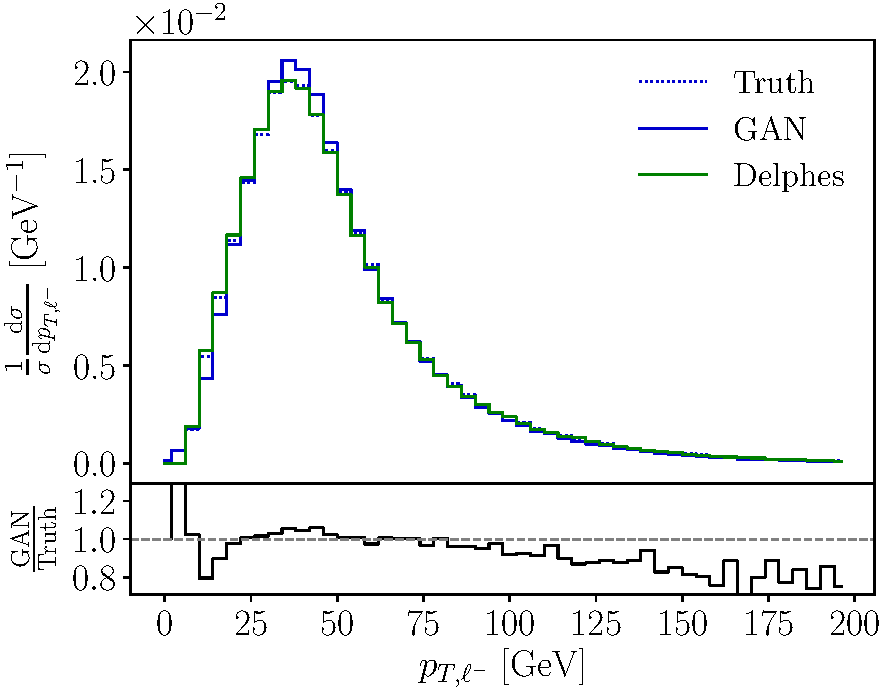
\includegraphics[page = 1, width=0.49\textwidth]{figures/cGAN/GAN_ratio}
\includegraphics[page = 4, width=0.49\textwidth]{figures/cGAN/GAN_ratio}
\caption{Example distributions for parton level truth, after
  detector simulation, and GANned back to parton level. The lower
  panels give the ratio of parton level truth and
  reconstructed parton level.}
\label{fig:distributions_GAN}
\end{figure}
%------------------------------------------------------------

For all GAN trainings we use a dataset of 300k events.
While the smearing of the lepton momenta is modest, 
the observed widths of the hadronically decaying $W$-boson will 
be much larger than the parton-level Breit-Wigner distribution. 
For this reason, we focus on showing hadronic observables to benchmark 
the performance of our set-up.

In Fig.~\ref{fig:distributions_GAN} we
compare true parton-level events to the GAN's output.  
We run the GAN on a set of statistically independent, 
but simulation-wise identical sets of detector-level events. 
Both, the relatively flat $p_{T,j_1}$ and the
peaked $m_{jj}$ distributions agree well between the true parton-level
events and the GAN-inverted sample, indicating that the model
is able to reproduce the parton level observables correctly.

This first approach only serves as a check that the training procedure of the
GAN leads to the correct outcome, as it suffers from severe limitations. 
First of all, we wish to invert the detector simulation stochastically, i.e. 
we want the full posterior distribution of possible parton level events
associated to a single detector level event. As this setting doesn't accommodate
any random input, and the generator itself is a deterministic map, this is 
not possible.
Secondly, the detector information is completely ignored by the model, 
as in the training batches of parton and detector get shuffled independently, 
and there's therefore no connection between each them. 
In order to illustrate this second point better, we invert an event sample which is not
statistically equivalent to the training data, specifically by testing the GAN on 
data covering only part of the detector-level phase space. 
We apply the two sets of jet cuts
%
\begin{alignat}{5}\tag{7}
&\text{Cut I}: & \quad
p_{T,j_1} &= 30~...~100~\gev
\label{eq:jetcut1a} \\\tag{8}
&\text{Cut II}: & \quad
p_{T,j_1} &= 30~...~60~\gev \quad \text{and} \quad p_{T,j_2} = 30~...~50~\gev \; ,
\label{eq:jetcut1b}
\end{alignat}
%
which leave us with 88\% and 38\% of events, respectively. This
approach ensures that the training has access to the full information,
while the test sample is a significantly reduced sub-set of the full
sample.

%------------------------------------------------------------
\begin{figure}[t]
\centering
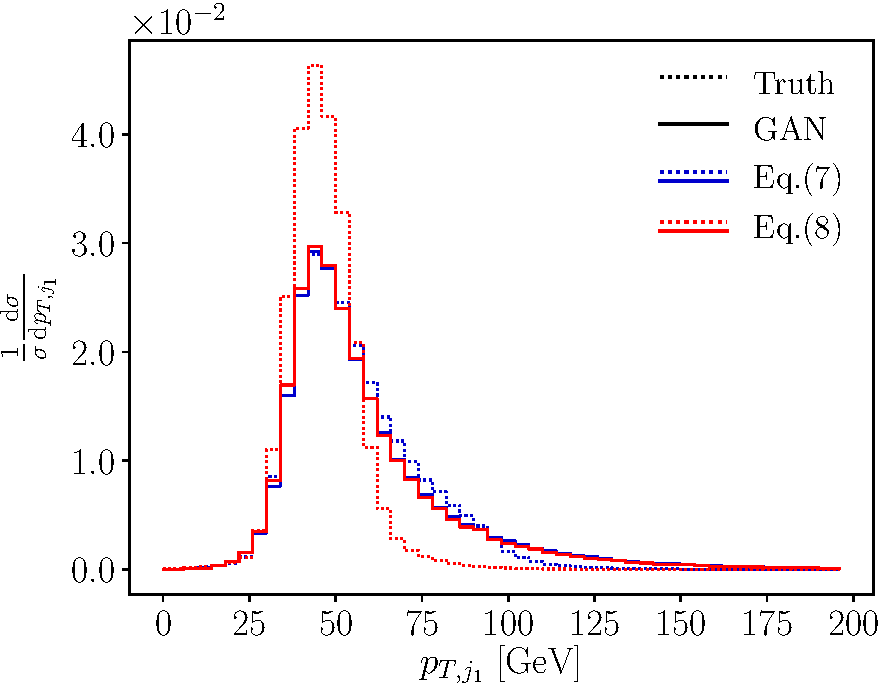
\includegraphics[page = 1, width=0.49\textwidth]{figures/cGAN/GAN_overlap}
\includegraphics[page = 2, width=0.49\textwidth]{figures/cGAN/GAN_overlap}
\caption{Parton level truth and GANned distributions when we train the
  GAN on the full data set but only unfold parts of phase space
  defined in Eq.\eqref{eq:jetcut1a} and Eq.\eqref{eq:jetcut1b}.}
\label{fig:distributions_GAN_sliced}
\end{figure}
%------------------------------------------------------------

In Fig.~\ref{fig:distributions_GAN_sliced} we show a set of kinematic
distributions with detector cuts propagated to the parton level. As
before, we compare the original parton-level shapes of the
distributions with the results from inverting the fast detector
simulation.  
We see that while there's a strong correlation in the paired dataset
used for the training, the model is completely insensitive to it, and 
simply reproduces the full parton level information.
This is clear indications that the naive GAN approach doesn't exploit 
the fact that parton and detector events are paired. We discuss a 
solution in the next section.

%%%%%%%%%%%%%%%%%%%%%%%%%%%%%%%%%%%%%%%%%%%%%%%%%%%%%%%%%
\subsection{Conditional GAN}
\label{sec:fcgan}

%------------------------------------------------------------
\begin{figure}[t]
\centering
%\definecolor{Gcolor}{HTML}{3b528b}
%\definecolor{Dcolor}{HTML}{e41a1c}

\definecolor{Gcolor}{HTML}{2c7fb8}
\definecolor{Dcolor}{HTML}{f03b20}

\tikzstyle{generator} = [thick, rectangle, rounded corners, minimum width=1.5cm, minimum height=1cm,text centered, draw=Gcolor]
\tikzstyle{discriminator} = [thick, rectangle, rounded corners, minimum width=1.5cm, minimum height=1cm,text centered, draw=Dcolor]
\tikzstyle{mmd} = [thick, rectangle, rounded corners, minimum width=1.5cm, minimum height=1cm,text centered, draw=black]
\tikzstyle{io} = [thick,circle, trapezium left angle=70, trapezium right angle=110, minimum width=1.2cm, minimum height=1cm, text centered, draw=black]

\tikzstyle{cond} = [thick, rectangle, dotted, rounded corners, minimum width=10.0cm, minimum height=2cm,text centered, draw=gray!50!black]

\tikzstyle{iodotted} = [thick, circle, trapezium left angle=70, trapezium right angle=110, minimum width=1.2cm, minimum height=1cm, text centered, draw=black, dotted]

\tikzstyle{process} = [thick, rectangle, minimum width=1cm, minimum height=1cm, text centered, draw=black]

\tikzstyle{xG} = [thick,rectangle, minimum width=2.2cm, minimum height=3cm, text depth= 2.2cm, draw=black]
\tikzstyle{s0} = [thick,rectangle, minimum width=2cm, minimum height=3cm, text centered]
\tikzstyle{s1} = [thick, dotted, rectangle, minimum width=1.6cm, minimum height=1.1cm, text centered, draw=black]


\tikzstyle{decision} = [thick,rectangle, minimum width=1cm, minimum height=1cm, text centered, draw=black]


\tikzstyle{dots} = [circle, minimum size=2pt, inner sep=0pt,outer sep=0pt, draw=Dcolor, fill = Dcolor]

\tikzstyle{arrow} = [thick,->,>=stealth]

\begin{tikzpicture}[node distance=2cm]


\node (generator) [generator] {$G$};
\node (random) [io, left of=generator, xshift=-0.2cm, yshift=0cm] {$\{ r \}$};
\draw [arrow, color=black] (random) -- (generator);
\node (xG) [io, right of = generator, xshift=1.0cm, yshift=0cm] {$\{x_G\}$};
\node (discriminator) [discriminator, right of = xG, xshift=1.0cm, yshift=0cm] {$D$};

\node (cond) [cond, above of = generator, xshift=1.5cm, yshift=0.5cm] {};
\node (condi) [above of = xG, xshift=1.9cm, yshift=1.2cm, color=gray!50!black] {Condition};

\node (xd) [io, above of = generator, xshift=0.cm, yshift=0.5cm] {$\{x_d\}$};
\node (xp) [io, below of = xG, xshift=0.5cm, yshift=0cm] {$\{x_p\}$};

\node (detector) [process, left of=xd, xshift=-0.2cm, yshift=0cm] {detector};
\node (parton) [process, left of=xp, xshift=-0.2cm, yshift=0cm] {parton};

\coordinate[ above of= discriminator, xshift=-0.1cm, yshift=0.5cm] (in1);
\draw [thick, color=black] (xd) -- (in1);
\draw [arrow, color=black] (in1) -- ([xshift=-0.1cm] discriminator.north);

\draw [arrow, color=black] (detector) -- (xd);
\draw [arrow, color=black] (parton) -- (xp);
\draw [arrow, color=black] (xd) -- (generator);
\draw [arrow, color=black] (xp) -- (discriminator);
\draw [arrow, color=Gcolor] (generator) -- (xG);
\draw [arrow, color=Gcolor] (xG) -- (discriminator);

\node (dloss) [process, right of=discriminator, xshift=0.5cm, yshift=0cm] {$L_{D}$};
\node (gloss) [process, below of=dloss, xshift=0.0cm, yshift=0cm] {$L_{G}$};
\node (mmd) [mmd, below of=discriminator, xshift=0.0cm, yshift=0cm] {MMD};

\draw [arrow, color=Gcolor] (discriminator) -- (gloss);
\draw [arrow, color=Dcolor] (discriminator) -- (dloss);

\coordinate[ above of = dloss, xshift=0cm, yshift=-1cm] (d1);
\coordinate[ above of = discriminator, xshift=0.1cm, yshift=-1cm] (d2);
\draw[thick, dashed, color=Dcolor] (dloss) -- (d1);
\draw[thick, dashed, color=Dcolor] (d1) -- (d2);
\draw[arrow, dashed, color=Dcolor] (d2) -- ([xshift=0.1cm] discriminator.north);

\draw[arrow, color=Gcolor] (xG) --  (mmd);
\draw[arrow, color=black] (xp) --  (mmd);
\draw[arrow, color=Gcolor] (mmd) --  (gloss);
%\draw[arrow, color=Gcolor] (xd) -- (mmd);


\coordinate[ below of = gloss, xshift=0cm, yshift=1.0cm] (out1);
\coordinate[ below of = generator, xshift=0cm, yshift=-1.0cm] (out2);
\draw[thick, dashed, color=Gcolor] (gloss) --  (out1);
\draw[thick, dashed, color=Gcolor] (out1) --  (out2);
\draw[arrow, dashed, color=Gcolor] (out2) --  (generator);








\end{tikzpicture}

\caption{Structure of our fully conditional FCGAN. The
  input $\{r\}$ describes a batch of random numbers and $\{ x_{G,d,p}
  \}$ denotes events sampled from the generator, detector-level data,
  or parton-level data. The blue (red) arrows indicate which
  connections are used in the training of the generator
  (discriminator).}
\label{fig:FCGAN}
\end{figure}
%------------------------------------------------------------

The issues highlighted in the previous section can be simultaneously solved
by switching to a conditional GAN set-up~\cite{cond_gan}, which we show
 in Fig.~\ref{fig:GANs}. First of all, we recover the physical intuition that
this entire mapping is statistical in nature by feeding the generator random
numbers $\{z\}$ sampled from a simple, fixed distribution, in our case a multivariate
Gaussian with zero mean and the identity as the covariance matrix. The input
is taken with the same dimensionality as the target space.
Secondly, the detector-level information $\{ x_d \}$ is used as an event-by-event conditional input
on the link between a set of random numbers and the parton-level
output, \ie $G( \{ r \}, \{ x_d \} ) = \{ x_G \}$. This way the conditional model
can generate parton-level events from random noise but still using the
detector-level information as input. 
%
%
%The idea behind the conditional set-up is not to learn a deterministic link between input
%and output samples, because we know that without an enforced structure
%in the weight or function space the generator does not benefit from
%the structured input. In other words, the network does not properly
%exploit the fact that the detector-level and parton-level data sets in
%the training sample are paired.  A second, related problem of the
%naive GAN is that once trained the model is completely deterministic,
%so each detector-level event will always be mapped to the same
%parton-level events. This goes against the physical intuition that
%this entire mapping is statistical in nature.

%------------------------------------------------------------

\begin{figure}[t]
\centering
\includegraphics[page = 2, width=0.49\textwidth]{figures/cGAN/cGAN_full_ratio}
\includegraphics[page = 3, width=0.49\textwidth]{figures/cGAN/cGAN_full_ratio} \\
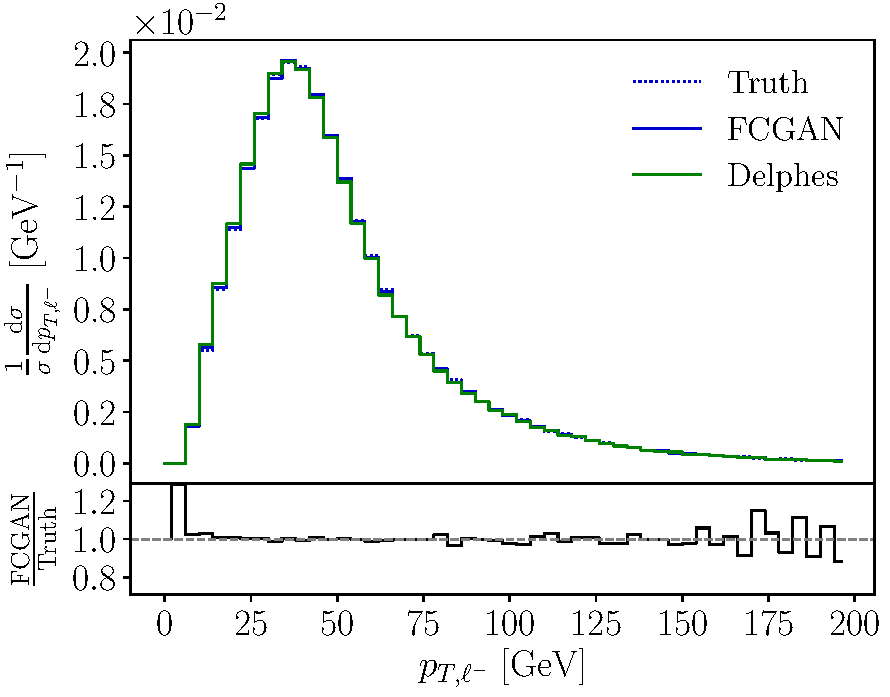
\includegraphics[page = 1, width=0.49\textwidth]{figures/cGAN/cGAN_full_ratio}
\includegraphics[page = 4, width=0.49\textwidth]{figures/cGAN/cGAN_full_ratio}
\caption{Example distributions for parton level truth, after detector
  simulation, and FCGANned back to parton level. The lower panels give
  the ratio of parton level truth and reconstructed parton level.  The
  lower panels give the deviation between parton level truth and
  reconstructed parton level. To be compared with the naive GAN
  results in Fig.~\ref{fig:distributions_GAN}.}
\label{fig:distributions_FCGAN}
\end{figure}
%------------------------------------------------------------

%------------------------------------------------------------
\begin{table}[b!]
\begin{small} \begin{center}
\begin{tabular}{l r | l r}
\toprule
Parameter              & Value   & Parameter              & Value  \\
\midrule
Layers & 12 & Batch size & 512 \\
Units per layer & 512 & Epochs & 1200\\
Trainable weights G & 3M  & Iterations per epoch & 500\\
Trainable weights D & 3M  & Number of training events & $3 \times 10^5$\\
\midrule
$\lambda_G$ & 1 \\
$\lambda_D$ & $10^{-3}$ \\
\bottomrule
\end{tabular}
\end{center} \end{small}
\caption{FCGAN setup.}
\label{tab:details}
\end{table}
%------------------------------------------------------------

In Fig.~\ref{fig:FCGAN} we introduce a fully conditional GAN
(FCGAN).
While the training procedure is identical, we need to modify the objective function as
%
\begin{align}
L_D \to L_D^\text{(FC)}= \left\langle - \log D\left(x, y\right) \right\rangle_{x \sim P_p, y \sim P_d} + \left\langle - \log\left( 1-D\left(x,y\right)\right) \right\rangle_{x \sim P_G, y \sim P_d} \; ,
\label{eq:D_closs}
\end{align}
%
and the regularized loss function changes accordingly,
%
\begin{align}
\begin{split}
L_D^\text{(reg)} \to L_D^\text{(reg,\,FC)} =
L_D^\text{(FC)}
&+ \lambda_D\,
\Langle \left(1- D(x,y)\right)^2 \vert \nabla \phi \vert^2 \Rangle_{x \sim P_p, y \sim P_d} \\
&+ \lambda_D\,
\Langle D\left(x,y\right)^2\, \vert \nabla \phi \vert^2 \Rangle_{x \sim P_G, y \sim P_d}  \; ,
\end{split}
\label{eq:Dcloss2}
\end{align}
%

again using the conventions of Ref.~\cite{gan_phasespace}. The
generator loss function now takes the form
%
\begin{align}
L_G\to L_G^\text{(FC)} = \left\langle - \log D\left(x,y\right) \right\rangle_{x \sim P_G, y \sim P_d} \; .
\label{eq:G_closs}
\end{align}
%
Note, that we do not build a conditional version of the MMD loss.  The
hyper-parameters of our FCGAN are summarized in
Tab.~\ref{tab:details}. Changing from a naive GAN to a
conditional GAN we have to pay a price in the structure of the
training sample. While the naive GAN only required event batches to be
matched between parton level and detector level, the training of the
FCGAN actually requires event-by-event matching.\medskip

In Fig.~\ref{fig:distributions_FCGAN} we compare the truth and the
generated events, trained on and applied to events covering the full
phase space. Compared to the naive GAN, inverting the detector effects
now works even better. The under-estimate of the GAN rate in tails no longer 
occurs for the FCGAN.  The reconstructed invariant
$W$-mass forces the network to dynamically generate a very narrow
physical width from a comparably broad Gaussian peak. Using our usual
MMD loss developed in Ref.~\cite{gan_phasespace} we reproduce the peak
position, width, and peak shape to about 90\%. We emphasize that
the MMD loss requires us to specify the relevant one-dimensional
distribution, in this case $m_{jj}$, but it then extracts the on-shell
mass or width dynamically. The multi-kernel approach we use in this
case is explained in the Appendix.

%------------------------------------------------------------
\begin{figure}[t]
\centering
\includegraphics[page = 2, width=0.49\textwidth]{figures/cGAN/cGAN_overlap_1}
\includegraphics[page = 3, width=0.49\textwidth]{figures/cGAN/cGAN_overlap_1} \\
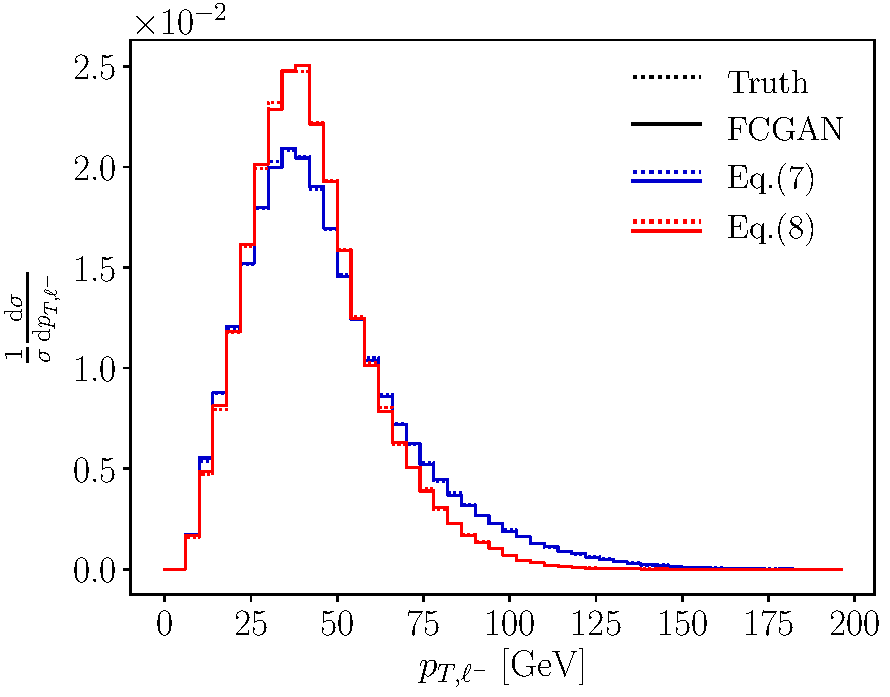
\includegraphics[page = 1, width=0.49\textwidth]{figures/cGAN/cGAN_overlap_1}
\includegraphics[page = 4, width=0.49\textwidth]{figures/cGAN/cGAN_overlap_1}
\caption{Parton level truth and FCGANned distributions when we train
  the GAN on the full data set but only unfold parts of phase space
  defined in Eq.\eqref{eq:jetcut1a} and Eq.\eqref{eq:jetcut1b}. To be
  compared with the naive GAN results in
  Fig.\ref{fig:distributions_GAN_sliced}.}
\label{fig:distributions_FCGAN_sliced_1}
\end{figure}
%------------------------------------------------------------

As for our naive ansatz we now test what happens to the network when
the training data and the test data do not cover the same phase space
region. We train using the entire phase space, but we then only
invert to the 88\% and 38\% of events passing the jet
cuts~I and~II defined in Eq.\eqref{eq:jetcut1a} and
Eq.\eqref{eq:jetcut1b}. We show the results in
Fig.~\ref{fig:distributions_FCGAN_sliced_1}. As observed before,
especially the jet cuts with only 40\% survival probability shape our
four example distributions. However, we see for example in the
$p_{T,jj}$ distribution that the inverted detector-level sample
reconstructs the patterns of the true parton-level events
perfectly. This comparison indicates that the FCGAN approach deals
with differences in the training and test samples very well.

%------------------------------------------------------------
\begin{figure}[t]
\centering
\includegraphics[page = 2, width=0.49\textwidth]{figures/cGAN/cGAN_overlap_2}
\includegraphics[page = 3, width=0.49\textwidth]{figures/cGAN/cGAN_overlap_2} \\
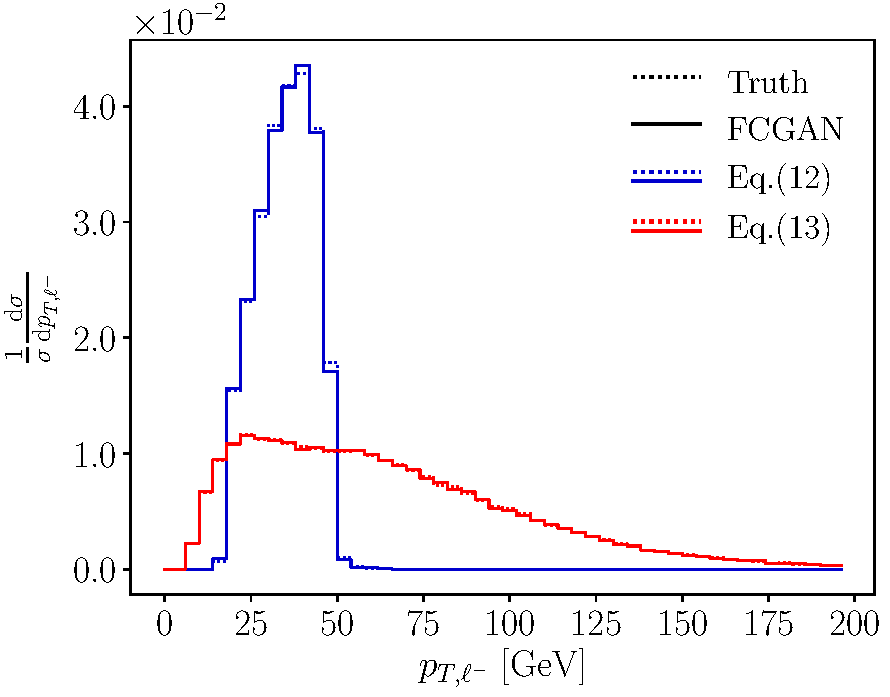
\includegraphics[page = 1, width=0.49\textwidth]{figures/cGAN/cGAN_overlap_2}
\includegraphics[page = 4, width=0.49\textwidth]{figures/cGAN/cGAN_overlap_2}
\caption{Parton level truth and FCGANned distributions when we train
  the GAN on the full data set but only unfold parts of phase space
  defined in Eqs.\eqref{eq:jetcut2a} and~\eqref{eq:jetcut2b}.}
\label{fig:distributions_FCGAN_sliced_2}
\end{figure}
%------------------------------------------------------------

In order to test to which degree the inversion holds, we move on to harsher 
cuts on the inclusive event sample. We start with
%
\begin{align}\tag{12}
\text{Cut III}: \quad p_{T,j_1}= 30~...~50~\gev
\quad p_{T,j_2} = 30~...~40~\gev
\quad p_{T,\ell^-} = 20~...~50~\gev \; ,
\label{eq:jetcut2a}
\end{align}
%
which $14\%$ of all events pass. In
Fig.~\ref{fig:distributions_FCGAN_sliced_2} we see that also for this
much reduced fraction of test events corresponding to the training
sample the FCGAN inversion reproduces the true distributions extremely
well, to a level where it appears not really relevant what fraction of
the training and test data correspond to each other.

Finally, we apply a cut which not only removes a large fraction of
events, but also cuts into the leading peak feature of the $p_{T,j_1}$
distribution and removes one of the side bands needed for an
interpolation,
%
\begin{align}\tag{13}
\text{Cut IV}: \quad  p_{T,j_1} > 60~\gev \; .
\label{eq:jetcut2b}
\end{align}
%
For this choice 39\% of all events pass, but we remove all events at
low transverse momentum, as can be seen from
Fig.~\ref{fig:distributions_FCGAN}. This kind of cut could therefore
be expected to break the unfolding. Indeed, the red lines in
Fig.~\ref{fig:distributions_FCGAN_sliced_2} indicate that we have
broken the $m_{jj}$ reconstruction through the FCGAN. However, all
other (shown) distributions still agree with the parton-level truth
extremely well. The problem with the invariant mass distribution is
that our implementation of the MMD loss is not actually
conditional. At this stage it means that, when pushed
towards its limits, the network will first fail to reproduce the
correct peak width in the $m_{jj}$ distribution, while all other
kinematic variables remain stable.\medskip

%------------------------------------------------------------
\begin{figure}[t]
\centering
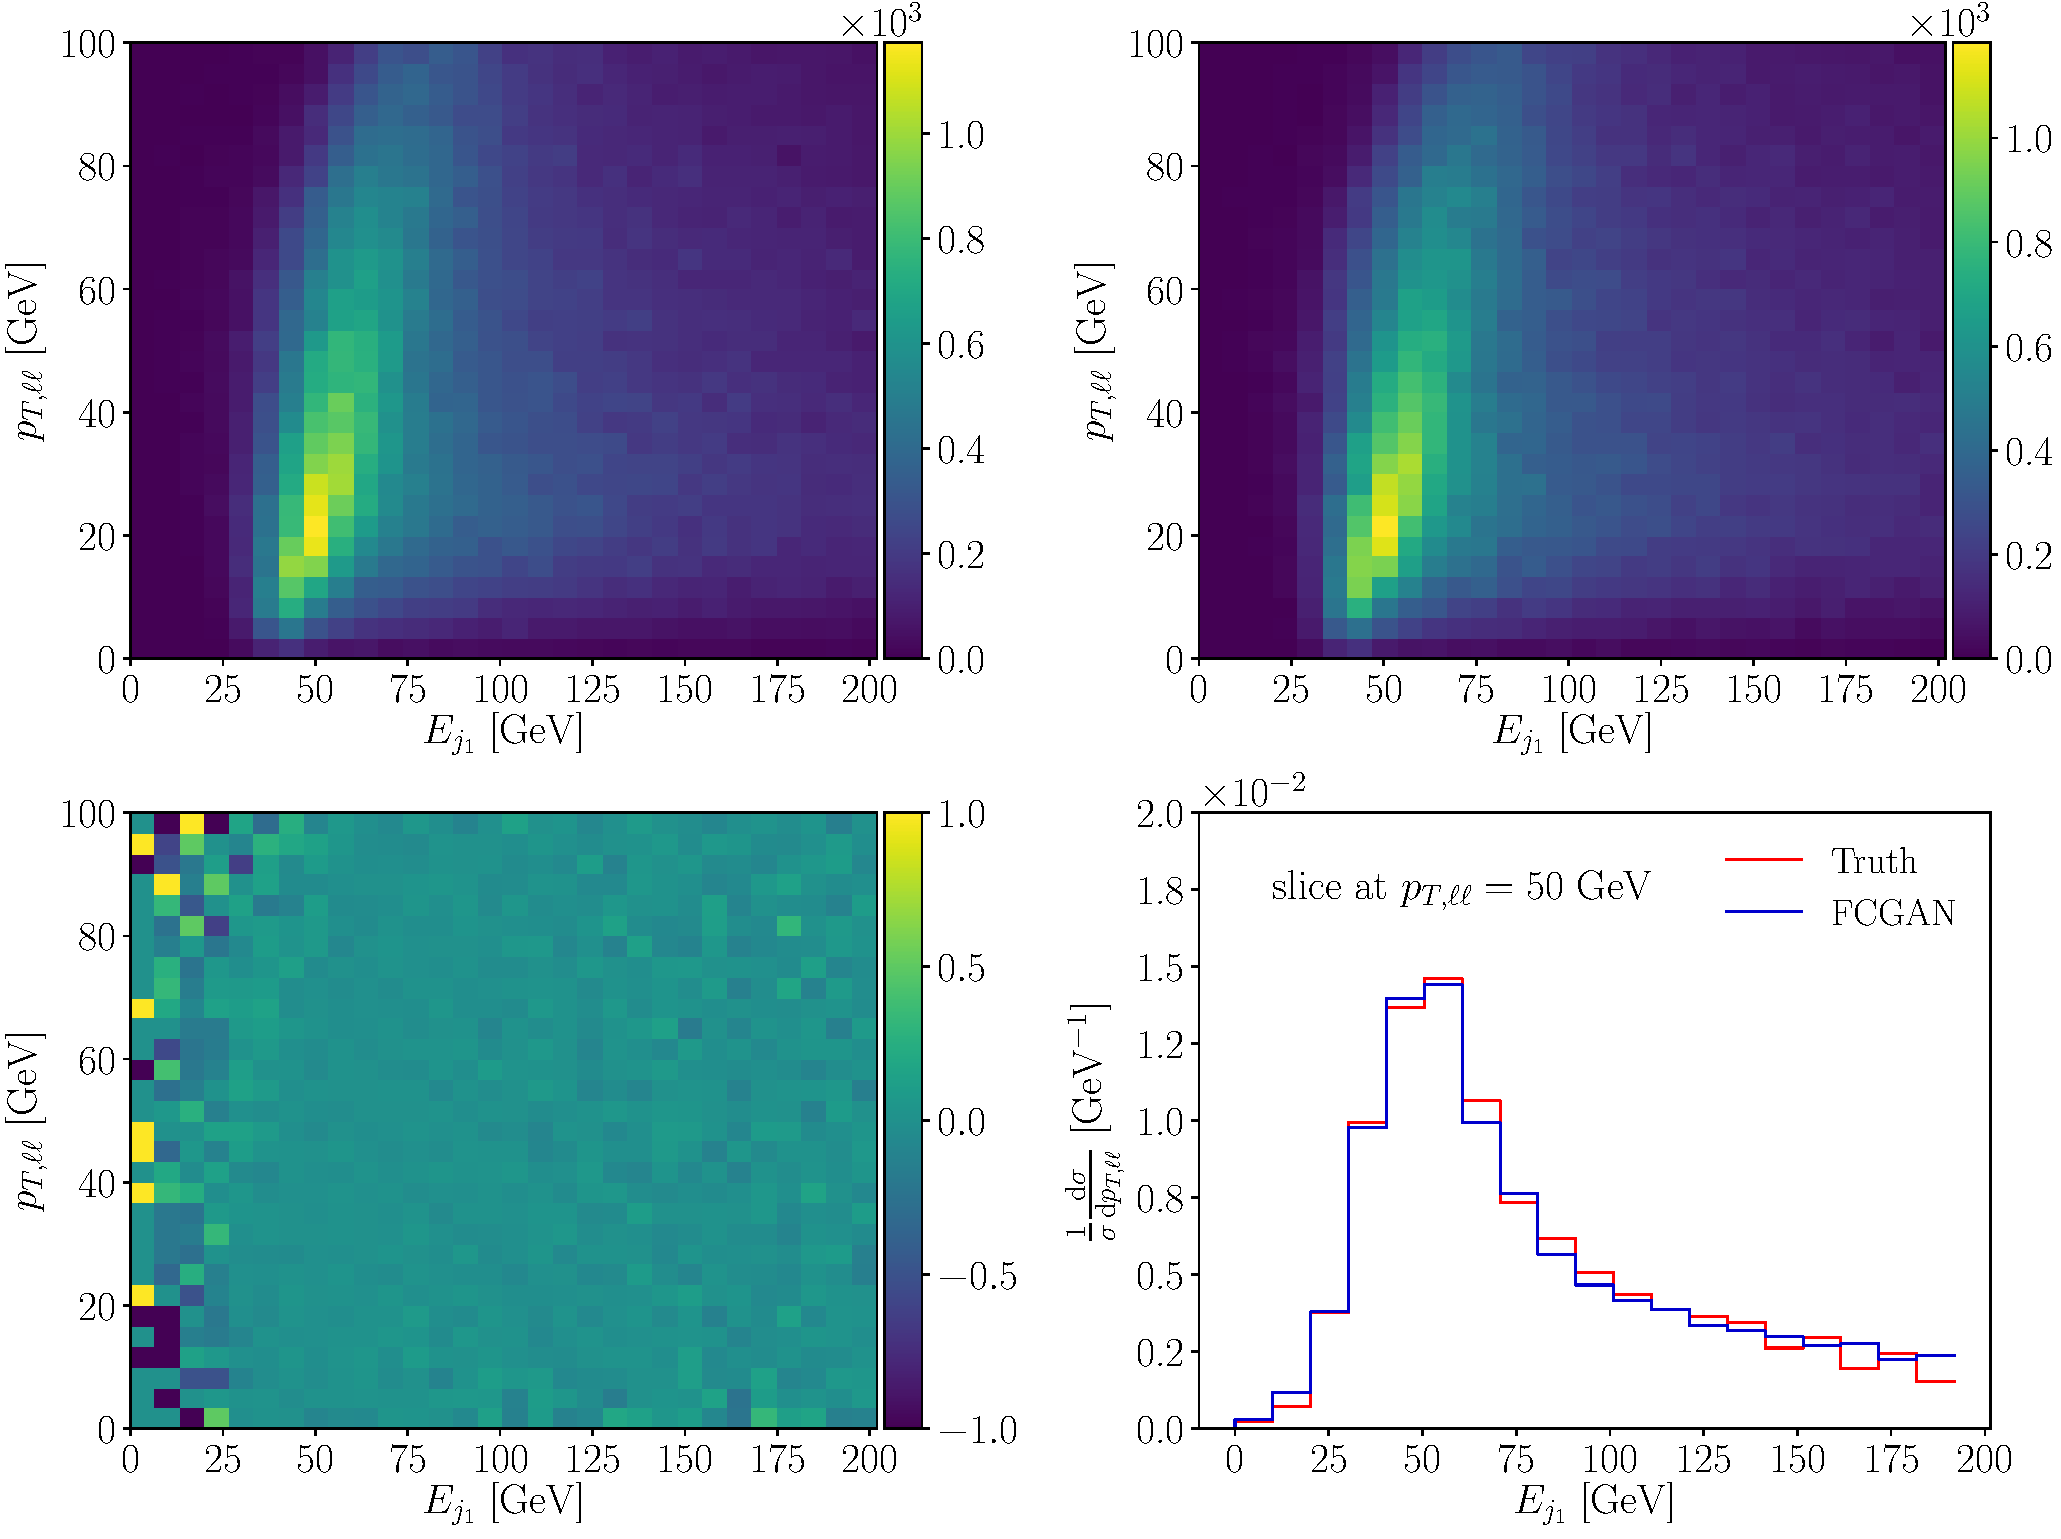
\includegraphics[width=0.98\textwidth]{figures/cGAN/cGAN_2d_corr}
\caption{Two-dimensional parton level truth (upper left) and FCGANned
  (upper right) distributions when we train the GAN on the full data
  set and unfold over the full phase space. The lower panels show the
  relative deviation between truth and FCGANned and the one-dimensional
  $E_{j_1}$ distribution along fixed $p_{T,\ell \ell}$.}
\label{fig:full_2d}
\end{figure}
%------------------------------------------------------------

Finally, just like in Ref.~\cite{gan_phasespace} we show 2-dimensional
correlations in Fig.~\ref{fig:full_2d}. We stick to applying the
network to the full phase space and show the parton level truth and
the FCGAN-inverted events in the two upper panels. Again, we see that
the FCGAN reproduces all features of the parton level truth with high
precision. The bin-wise relative deviation between the two 2-dimensional
distributions only becomes large for small values of $E_{j_1}$, where
the number of training events is extremely small.

%%%%%%%%%%%%%%%%%%%%%%%%%%%%%%%%%%%%%%%%%%%%%%%%%%%%%%%%%
\subsection{New physics injection}
\label{sec:closure}

As discussed before, unfolding to a hard process is necessarily
model-dependent. Until now, we have always assumed the Standard Model
to correctly describe the parton-level and detector-level events. 
An obvious question is what happens if we train our FCGAN on Standard
Model data, but apply it to a different hypothesis. This challenge
becomes especially interesting if this alternative hypothesis differs
from the Standard Model in a local phase space effect. It then allows
us to test if the generator networks maps the parton-level and
detector-level phase spaces in a structured manner. Such features of
neural networks are at the heart of all variational constructions, for
instance variational autoencoders which are structurally close to
GANs. 

To this end we add a fraction of resonant $W'$ events from a
triplet extension of the Standard Model~\cite{Biekoetter:2014jwa},
representing the hard process
%
\begin{align}
p p
\to {W'}^*
\to Z W^\pm
\to (\ell^- \ell^+) \; (j j )
\end{align}
%
to the test data.  We simulate these events with madgraph using the
model implementation of Ref.~\cite{Brehmer:2015rna} and denote the new
massive charged vector boson with a mass of 1.3~TeV and a width of
15~GeV as $W'$. For the test sample we combine the usual Standard
Model sample with the $W'$-sample in proportions $90\% - 10\%$.  The
other new particles do not appear in our process to leading order.
Because we want to test how well the GAN maps local phase space
structures onto each other, we deliberately choose a small width
$\Gamma_{W'}/M_{W'}\sim 1\%$, not exactly typical for such strongly
interacting triplet extensions.

%------------------------------------------------------------
\begin{figure}[t]
\centering
\includegraphics[page = 9, width=0.49\textwidth]{figures/cGAN/6f_plots_mix}
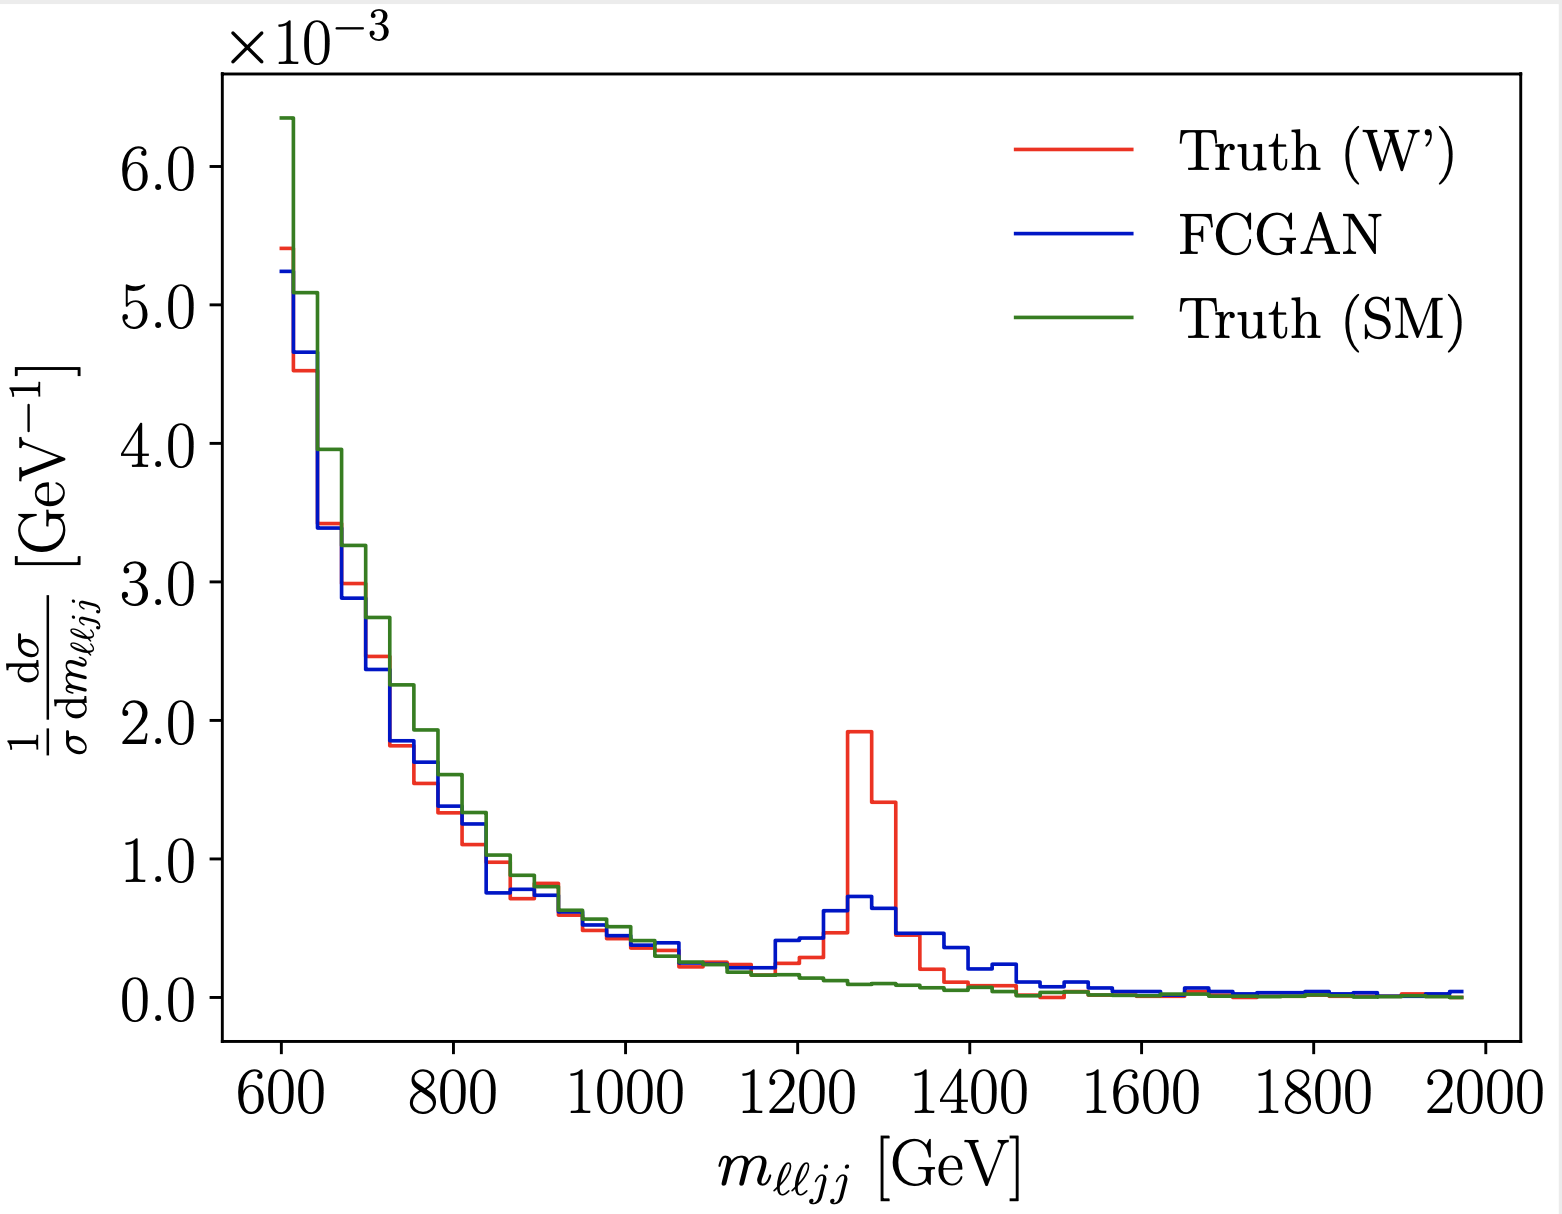
\includegraphics[page = 1, width=0.49\textwidth]{figures/cGAN/6f_plots_mix}\\
\includegraphics[page = 17, width=0.49\textwidth]{figures/cGAN/6f_plots_mix}
\includegraphics[page = 18, width=0.49\textwidth]{figures/cGAN/6f_plots_mix}
\caption{Parton level truth and FCGANned distributions when we train
  the network on the Standard Model only and unfold events with an
  injection of $10\%$ $W'$ events. The mass of the
  additional $s$-channel resonance is 1.3~TeV.}
\label{fig:w_prime}
\end{figure}
%------------------------------------------------------------

The results for this test are shown in Fig.~\ref{fig:w_prime}. First,
we look at transverse momentum distribution of final-state particles,
which are hardly affected by the new heavy resonance. Both, the
leading jet and the lepton distributions are essentially identical for
both truth levels and the FCGAN output. The same is true for the
invariant mass of the hadronically decaying $W$-boson, which
nevertheless provides a useful test of the stability of our training
and testing.

Finally, we show the reconstructed $W'$-mass in the lower-right
pane. Here we see the different (normalized) truth-level distributions
for the Standard Model and the $W'$-injected sample. The FCGAN,
trained on the Standard Model, keeps track of local phase space
structures and reproduces the $W'$ peak faithfully. It also learn the
$W'$-mass as the central peak position very well. The only issue is
the $W'$-width, which the network over-estimates. However, we know
already that dynamically generated width distributions are a challenge
to GANs and require for instance an MMD loss.  Nevertheless,
Fig.~\ref{fig:w_prime} clearly shows that GAN unfolding shows a high
degree of model independence, making use of local structures in the
mapping between the two phase spaces. We emphasize that the additional
mass peak in the FCGANned events is not a one-dimensional feature, but
a localized structure in the full phase space. This local structure is
a feature of neural networks which comes in addition to the known
strengths in interpolation.

%%%%%%%%%%%%%%%%%%%%%%%%%%%%%%%%%%%%%%%%%%%%%%%%%%%%%%%%%

\section{INN unfolding}
\label{sec:inn}

In Sec.~\ref{sec:ganunfolding} we have introduced and developed the idea
of inverting Monte Carlo simulations using a GAN. However, it should be 
clear from Sec.~\ref{intro:normflow} that an invertible model is a more
natural tool to use, as the task we wish to solve consists precisely of 
inverting a well known forward simulation. We will show in this section how
the intuition built with the conditional GAN provides us with a useful 
guideline.

We introduce the conditional INN in two steps, starting with the
non-conditional, standard set-up. The construction of the INN we use in
our analysis combines two goals~\cite{inn}:
%
\begin{enumerate}
\item the mapping from input to output is invertible and the Jacobians
  for both directions are tractable;
\item both directions can be evaluated efficiently. This second
  property goes beyond some other implementations of normalizing
  flow~\cite{nflow1,nflow_review}.
\end{enumerate}
%
While the final aim is not to actually evaluate our INN in both directions, we will
see that these networks can be extremely useful to invert a stochastic
process like detector smearing.

In Sec.~\ref{sec:inn_cond} we will show how the conditional INN
retains a proper statistical notion of the inversion to parton level
phase space.  This avoids a major weakness of standard unfolding
methods, namely that they only work on large enough event samples
condensed to one-dimensional or two-dimensional kinematic
distributions. This could be a missing transverse energy distribution
in mono-jet searches or the rapidities and transverse momenta in top
pair production. To avoid systematics or biases in the full phase
space coverage required by the matrix element method, the unfolding
needs to construct probability distributions in parton-level phase
space, including small numbers of events in tails of kinematic
distributions.

%%%%%%%%%%%%%%%%%%%%%%%%%%%%%%%%%%%%%%%%%%%%%%%%%%%%%%%%%
\subsection{Naive INN}
\label{sec:inn_base}

%------------------------------------------------------------
\begin{figure}[t]
\centering

%\definecolor{Gcolor}{HTML}{3b528b}
%\definecolor{Dcolor}{HTML}{e41a1c}

\definecolor{Gcolor}{HTML}{2c7fb8}
\definecolor{Dcolor}{HTML}{f03b20}


\tikzstyle{INN} = [thick, rectangle, rounded corners, minimum width=2.5cm, minimum height=3.5cm,text centered, draw=Gcolor]
\tikzstyle{preprocessor} = [thick, rectangle, rounded corners, minimum width=1.5cm, minimum height=1cm,text centered, draw=Dcolor]
\tikzstyle{mmd} = [thick, rectangle, rounded corners, minimum width=1.5cm, minimum height=1cm,text centered, draw=black]
\tikzstyle{io} = [thick,circle, minimum width=1.2cm, minimum height=1.2cm, text centered, draw=black]

\tikzstyle{cond} = [thick, rectangle, dotted, rounded corners, minimum width=10.0cm, minimum height=2cm,text centered, draw=gray!50!black]

\tikzstyle{iodotted} = [thick, circle, minimum width=1.2cm, minimum height=1cm, text centered, draw=black, dotted]

\tikzstyle{process} = [thick, rectangle, minimum width=1cm, minimum height=1cm, text centered, draw=black]

\tikzstyle{xG} = [thick,rectangle, minimum width=2.2cm, minimum height=3cm, text depth= 2.2cm, draw=black]
\tikzstyle{s0} = [thick,rectangle, minimum width=2cm, minimum height=3cm, text centered]
\tikzstyle{s1} = [thick, dotted, rectangle, minimum width=1.6cm, minimum height=1.1cm, text centered, draw=black]


\tikzstyle{decision} = [thick,rectangle, minimum width=1cm, minimum height=1cm, text centered, draw=black]


\tikzstyle{dots} = [circle, minimum size=2pt, inner sep=0pt,outer sep=0pt, draw=Dcolor, fill = Dcolor]

\tikzstyle{arrow} = [thick,->,>=stealth]

\begin{tikzpicture}[node distance=2cm]


\node (INN) [INN] {INN};

\node (xG) [io, left of = INN, xshift=-0.8cm, yshift=1cm] {$\{\tilde x_{p}, \tilde r_{p}\}$};
\node (rG) [io, right of = INN, xshift=0.8cm, yshift=-1cm] {$\{\tilde x_{d}, \tilde r_{d}\}$};


\node (xp) [io, left of = INN, xshift=-0.8cm, yshift=-1cm] {$\{x_p, r_p\}$};
\node (parton) [process, below of=xp, xshift=0cm, yshift=0cm] {parton};
\node (mmd) [mmd, left of=xp, xshift=0.0cm, yshift=1cm] {$L_\text{MMD, MSE}$};

\node (random) [io, right of=INN, xshift=0.8cm, yshift=1cm] {$\{ x_d, r_d \}$};
\node (detector) [process, above of=random, xshift=0cm, yshift=0cm] {detector};
\node (gauss) [mmd, right of=rG, xshift=0.0cm, yshift=1cm] {$L_\text{MMD, MSE}$};


%\node (cond) [cond, above of = xG, xshift=1.5cm, yshift=-0.1cm] {};
%\node (condi) [above of = xG, xshift=1.9cm, yshift=0.5cm, color=gray!50!black] {Condition};

%\node (preprocessor) [preprocessor, above of=INN, xshift=0cm, yshift=0.5cm] {Subnet};
%\node (xd) [io, left of = preprocessor, xshift=-0.5cm, yshift=0cm] {$\{x_d\}$};
%\node (detector) [process, left of=xd, xshift=-0.2cm, yshift=0cm] {detector};

\coordinate[ right of = rG, xshift=0cm, yshift=0cm] (Gin1);
\coordinate[ right of = random, xshift=0cm, yshift=0cm] (Gin2);

\coordinate[ left of = xG, xshift=0cm, yshift=0cm] (MMDin1);
\coordinate[ left of = xp, xshift=0cm, yshift=0cm] (MMDin2);



%\draw [arrow, color=black] ([yshift=0em]random.west) -- ([yshift=1.5em]INN.east);
%\draw [arrow, color=black] ([yshift=-1.5em]INN.east) -- (rG.west);
%\draw [arrow, color=black] ([yshift=1.5em]INN.west) -- (xG.east);
%\draw [arrow, color=black] ([yshift=0em]xp.east) -- ([yshift=-1.5em]INN.west);

\draw [arrow, color=black] ([yshift=0em]parton.north) -- ([yshift=0em]xp.south);
\draw [arrow, color=black] ([yshift=0em]detector.south) -- ([yshift=0em]random.north);

\draw [thick, color=Gcolor] ([yshift=0em]xp.west) -- ([yshift=0em]MMDin2);
\draw [arrow, color=Gcolor] ([yshift=0em]MMDin2) -- ([yshift=0em]mmd.south);
\draw [thick, color=Gcolor] ([yshift=0em]xG.west) -- ([yshift=0em]MMDin1);
\draw [arrow, color=Gcolor] ([yshift=0em]MMDin1) -- ([yshift=0em]mmd.north);

\draw [thick, color=Gcolor] ([yshift=0em]random.east) -- ([yshift=0em]Gin2);
\draw [arrow, color=Gcolor] ([yshift=0em]Gin2) -- ([yshift=0em]gauss.north);
\draw [thick, color=Gcolor] ([yshift=0em]rG.east) -- ([yshift=0em]Gin1);
\draw [arrow, color=Gcolor] ([yshift=0em]Gin1) -- ([yshift=0em]gauss.south);

%\draw [arrow, color=black] ([yshift=0em]detector.east) -- ([yshift=0em]xd.west);
%\draw [arrow, color=black] ([yshift=0em]xd.east) -- ([yshift=0em]preprocessor.west);
%\draw [arrow, color=black] ([yshift=0em]preprocessor.south) -- ([yshift=0em]INN.north);

%\draw[arrow, thick, color=Gcolor] (random.west) -- (xG.east);
\draw[arrow, color=Gcolor] (random.west) --  node[scale=0.8, sloped, anchor=center, above, color=Gcolor]{$\bar{g}(x_d, r_d)$} ([yshift=0cm]xG.east);
%\draw[arrow, thick, color=Gcolor] ([yshift=1cm]INN.west) -- (xG.east);
%\draw[arrow, thick, color=Gcolor] (xp.east) -- (rG.west);
%\draw[arrow, thick, color=Gcolor] (xp.east) -- ([yshift=-1cm]INN.west);
\draw[arrow, color=Gcolor] ([yshift=0cm]xp.east) --  node[scale=0.8, sloped, anchor=center, above, color=Gcolor]{$g(x_p, r_p)$} (rG.west);



\draw[arrow, thick, dashed, color=black] (mmd) -- (INN.west);
\draw[arrow, thick, dashed, color=black] (gauss) -- (INN.east);


\end{tikzpicture}

\caption{Structure of INN. The $\{ x_{d,p} \}$ denote detector-level
  and parton-level events, $\{ r_{d,p} \}$ are random numbers to match
  the phase space dimensionality. A tilde indicates the INN
  generation.}
\label{fig:inn}
\end{figure}
%------------------------------------------------------------

While it is clear from our discussion in Sec.~\ref{sec:ganunfolding} that a
standard INN will not serve our purpose, we still describe it in some
detail before we extend it to a conditional network.  
Following the conventions of our GAN analysis and in analogy to Eqs.\eqref{eq:toy1}
to \eqref{eq:toy3} we define the network input as a vector of hard
process information $x_p \in R^{D_p}$ and the output at detector level
via the vector $x_d \in \mathbb{R}^{D_d}$. 
as the INN is a change of variable, the input and output dimensionalities must be
the same. If the dimensionality of the spaces are such that $D_p < D_d$ 
we can add a noise vector $r$ with dimension
$D_d-D_p$ to define the bijective, invertible transformation,
%
\begin{align}
\begin{pmatrix} x_p \\ r \end{pmatrix}
\stackrel[\leftarrow \; \text{unfolding}: \bar{g}]{\textsc{Pythia,Delphes}: g \rightarrow}{\xleftrightarrow{\hspace*{3.5cm}}}
 x_d  \; .
\label{eq:mapping}
\end{align}
%
A correctly trained network $g$ with the parameters $\theta$
then reproduces $x_d$ from the combination $x_p$ and $r$. Its inverse
$\bar{g}$ instead reproduces the combination of $x_p$ and $r$ from $x_d$.

We have introduced in Sec.~\ref{intro:normflow} the general features of 
invertible models, i.e. models that learn both directions of the bijective mapping in parallel
and encodes them into one network as illustrated in Fig.~\ref{fig:inn} .
In particular, we have explained how we can think of an INN as the composition
of multiple copies of a single base function with the required properties
of invertibility and cheap Jacobian.
For our INN we have chosen invertible coupling layers~\cite{coupling1,coupling2}
based on dimensional partitioning.  For
notational purposes we ignore the random numbers in
Eq.\eqref{eq:mapping} and assume that this layer links an input vector
$x_p$ to an output vector $x_d$ after splitting both of them in
halves, $x_{p,i}$ and $x_{d,i}$ for $i=1,2$. The relation between
input and output is given by a sub-network, which encodes arbitrary
functions $s_{1,2}$ and $t_{1,2}$.  Using an element-wise
multiplication~$\odot$ and sum one could for instance define an output
$x_{d,1}(x_p) = x_{p,1} \odot s_2(x_{p,2}) + t_2(x_{p,2})$. 
In order to avoid numerical instabilities caused by the division with 
$s(x)$ in the inverse direction, we include an exponential to obtain
%
\begin{align}
\begin{pmatrix} x_{d,1} \\ x_{d,2} \end{pmatrix} =
\begin{pmatrix}
x_{p,1} \odot e^{s_2(x_{p,2})} + t_2(x_{p,2}) \\
x_{p,2} \odot e^{s_1(x_{d,1})} + t_1(x_{d,1})
\end{pmatrix}
\hspace{0.5em} \Leftrightarrow \hspace{0.5em}
\begin{pmatrix} x_{p,1} \\ x_{p,2} \end{pmatrix} =
\begin{pmatrix}
(x_{d,1} - t_2(x_{p,2})) \odot e^{-s_2(x_{p,2})} \\
(x_{d,2} - t_1(x_{d,1})) \odot e^{-s_1(x_{d,1})}
\end{pmatrix} \; .
\label{eq:layers}
\end{align}
%
By construction, this inversion works independent of the form of $s$
and $t$. If we write the coupling block function as $g(x_p) \sim x_d$,
again omitting the random numbers $r$, the Jacobian of the network
function has a triangular form
%
\begin{align}
\frac{\partial g(x_p)}{\partial x_p} =
\begin{pmatrix}
\text{diag } e^{s_2(x_{p,2})} & \text{finite} \\
0 & \text{diag } e^{s_1(x_{d,1})}
\end{pmatrix} \; ,
\label{eq:jacob}
\end{align}
%
so its determinant is easy to compute. Such coupling layer
transformations define the normalizing flow, when we view it
as transforming an initial probability density into a very general
form of probability density through a series of invertible steps. We
can relate the two probability densities as long as the Jacobians of
the individual layers can be efficiently calculated.

Since the first use of the invertible coupling layer, much effort has
gone into improving its efficiency. The All-in-One (AIO) coupling
layer includes two features, introduced by Ref.~\cite{coupling2} and
Ref.~\cite{glow}. The first modification replaces the transformation
of $x_{p,2}$ by a permutation of the output of each layer. Due to the
permutation each component still gets modified after passing through
several layers. The second modification includes a global affine transformation
to include a global bias and linear scaling that maps $x \rightarrow s
x + b$. Finally, we apply a bijective soft clamping after the
exponential function in Eq.\eqref{eq:layers} to prevent instabilities
from diverging outputs.

The INN in our simplified example combines three contributions to the
loss function. First, it tests if in the \textsc{Delphes} direction of
Eq.\eqref{eq:mapping} we indeed find $g(x_p) = x_d$ via the mean
squared error (MSE) function. While this is theoretically sufficient
to obtain the inverse function, also testing the inverse direction
$\bar{g}(x_d) = x_p$ greatly improves the efficiency and stability of
the training. Third, to resolve special sharp features like the
invariant mass of intermediate particles we use the MMD loss introduced 
in Sec.~\ref{sec:ganunfolding}. 
%Because we will also use the MMD in another function
%function~\cite{gan_phasespace} we review it briefly. An MMD loss
%allows us to compare any pre-defined distribution. For a relativistic
%phase space a critical narrow phase space feature is the invariant
%mass of intermediate particles. We can force the network to consider
%this one-dimensional distribution of the 4-vectors $x_p$ for batches
%of parton-level and detector-level events,
%%
%\begin{align}
%\text{MMD} =
%\left[ \langle k\left(x,x'\right)\rangle_{x,x' \sim P_p}
%     + \langle k\left(y,y'\right)\rangle_{y,y' \sim P_d}
%     - 2 \langle k\left(x,y \right)\rangle_{x\sim P_p,y \sim P_d} \right]^{1/2} \; .
%\label{eq:MMD2}
%\end{align}
%%
%In Refs.~\cite{gan_phasespace} and~\cite{fcgan} we compare common
%choices, like Gaussian or Breit-Wigner kernels
%%
%\begin{align}
%k_\text{Gauss} \left(x,y\right) = \exp \frac{- \left(x - y\right)^2}{2 \sigma^2}
%\qquad \text{or} \qquad
%k_\text{BW}\left(x,y\right) = \frac{\sigma^2}{\left(x - y\right)^2 + \sigma^2}
%\label{eq:kernels2}
% \end{align}
%%
%with a fixed or variable width $\sigma$~\cite{fcgan}. 
For the INN architecture the Breit-Wigner kernel is the best choice to analyze the
distribution of the random numbers as part of the loss
function~\cite{inn}.

%------------------------------------------------------------
\begin{figure}[t]
%\centering
\includegraphics[page=25, width=0.48\textwidth]{figures/cINN/INN_noE}
\includegraphics[page=25, width=0.48\textwidth]{figures/cINN/INN_FineTune} \\
\includegraphics[page=26, width=0.48\textwidth]{figures/cINN/INN_noE}
\includegraphics[page=26, width=0.48\textwidth]{figures/cINN/INN_FineTune} \\
\includegraphics[page=32, width=0.48\textwidth]{figures/cINN/INN_noE}
\includegraphics[page=32, width=0.48\textwidth]{figures/cINN/INN_FineTune}
\caption{INN-generated $p_{T,q}$ and $M_{W,\text{reco}}$ distributions from a
  naive INN (left) and the noise-extended eINN (right). In green we
  compare the detector-level truth to INNed events transformed from
  parton level. In blue we compare the parton-level truth to INNed
  events transformed from detector level. The secondary panels show
  the ratio of INNed events over parton-level truth. More
  distributions can be found in the pdf files submitted to the arXiv.}
\label{fig:UnfoldCurve}
\end{figure}
%------------------------------------------------------------

We now use the INN network to map parton-level events to
detector-level events or vice-versa. In a statistical analysis we then
use standard kinematic distributions and compare the respective truth
and INN-inverted shapes for both directions. The left panels of
Fig.~\ref{fig:UnfoldCurve} shows the transverse momentum distributions
of the two jets and their invariant mass for both directions of the
INN. The truth events at parton level and at detector level are marked
as dashed lines. Starting from each of the truth events we can apply
the INN describing the detector effects as $x_d = g(x_p)$ or unfolding
the detector effects as $x_p = \bar{g}(x_d)$ in
Eq.\eqref{eq:mapping}. The corresponding solid lines have to be
compared to the dotted truth lines, where we need to keep in mind that
at the parton level the relevant objects are quarks while at the
detector level they are jets.

For the leading jet the truth and INN-generated detector-level agree very
well, while for the second jet the naive INN fails to capture the hard
cut imposed by the jet definition. 
For the invariant mass we find that
the smearing due to the detector effects is reproduced well with some
small deviations in the tails. In the unfolding direction both $p_T$
distributions follow the parton level truth. The only difference is a
systematic lack of events in the tail for the second quark. This is
especially visible in the ratio of the INN-unfolded events and the
parton-level truth, indicating that also at small $p_T$ the network
does not fill the phase space sufficiently. Combining both directions
we see that in forward direction the INN produces a too broad
$p_T$-distribution, the unfolding direction of the INN produces a too
narrow distribution.  The conceptual advantage of the INN actually
implies a disadvantage for the inversion of particular difficult
features.  Finally, the invariant mass of the $W$ is reproduced
perfectly without any systematic deviation.

%%%%%%%%%%%%%%%%%%%%%%%%%%%%%%%%%%%%%%%%%%%%%%%%%%%%%%%%%
\subsection{Noise-extended INN}
\label{sec:inn_noise}

While our simplified example in the previous section shows the potential
 of INNs, it fails to incorporate key aspects of the physical
process.  First of all, the number of degrees of freedom is not
actually the same at parton level and at detector level. External
partons are on their mass shell, while jets come with a range of jet
masses. This mismatch becomes crucial when we include missing
transverse momentum in the signature.  We generally need fewer
parameters to describe the partonic scattering than the detector-level
process.  For a fixed set of parton-level momenta we usually smear
each momentum component to simulate the detector measurement. These
additional degrees of freedom are of stochastic nature, so adding
Gaussian random variable on the parton side of the INN could be a
first step to address this problem.

To also account for potentially unobservable degrees of freedom at the
parton level we extend each side of the INN by a random number vector.
The mapping in Eq.\eqref{eq:mapping} now includes two random number
vectors with dimensions $D_{r_d} = D_p$ and $D_{r_p} = D_d$,
%
\begin{align}
\begin{pmatrix} x_p \\ r_p \end{pmatrix}
\stackrel[\leftarrow \; \text{unfolding}: \bar{g}]{\textsc{Pythia,Delphes}: g \rightarrow}{\xleftrightarrow{\hspace*{3.5cm}}}
\begin{pmatrix} x_d \\ r_d \end{pmatrix} \; .
\label{eq:mappingnoise}
\end{align}
%
In addition, a pure MSE loss can not capture the fact that the
additional noise generates a distribution of detector-level events
given fixed parton momenta. It would just predict a mean value of
this distribution and minimize the effect of the noise. A better
solution is an MMD loss for each degree of freedom in the event and
the masses of intermediate particles, as well as the Gaussian random
variables. On the side of the random numbers this MMD loss ensures
that they really only encode noise. Again it is beneficial for the
training to use the inverse direction and apply additional MMD
losses to the parton level events as well as the corresponding
Gaussian inputs.  Finally we add a weak MSE loss on the four vectors
of each side to stabilize the training.

In the right panels of Fig.~\ref{fig:UnfoldCurve} we show results for
this noise-extended INN (eINN). The generated distributions are similar to
the naive INN case and match the truth at the parton level. A notable
difference appears in the second jet, the weak spot of the naive
INN. The additional random numbers and MMDs provide more freedom to
generate the peak in the forward direction and also improve the
unfolding in the low-$p_T$ and high-$p_T$ regimes.\bigskip

%------------------------------------------------------------
\begin{figure}[t]
\includegraphics[page=9, width=0.48\textwidth]{figures/cINN/point1_inn_fcgan}
\includegraphics[page=20, width=0.48\textwidth]{figures/cINN/CalibrationCurveINNFCGAN}
\caption{Left: illustration of the statistical interpretation of
  unfolded events for one event. Right: calibration curves for
  $p_{T,q_1}$ extracted from the FCGAN and the noise-extended eINN.}
\label{fig:quantile1}
\end{figure}
%------------------------------------------------------------

The noise extension allows for a
statistic interpretation of the generated distributions and a test of
the integrity of the INN-inverted distributions. In the left panel of
Fig.~\ref{fig:quantile1} we illustrate the goal of the statistical
treatment: we start from a single event at the detector level and
generate a set of unfolded events. For each of them we evaluate for
instance $p_{T,q_1}$. Already in this illustration we see that the GAN
output is lacking a statistical behaviour at the level of individual
events, while the noise-extended eINN returns a reasonable
distribution of unfolded events.

To see if the width of this INN output is correct we take 1500
parton-level and detector-level event pairs and unfold each event 60
times, sampling over the random variables. This gives us 1500
combinations like the one shown in the left panel of
Fig.~\ref{fig:quantile1}: a single parton-level truth configuration
and a distribution of the INNed configuration. To see if the central
value and the width of the INNed distribution can be interpreted
statistically as a posterior probability distribution in parton phase
space we analyse where the truth lies within the INN distribution for
each of the 1500 events.  For a correctly calibrated curve we start
for instance from the left of the kinematic distribution and expect
10\% of the 1500 events in the 10\% quantile of the respective
probability distribution, 20\% of events in the 20\% quantile, etc.
The corresponding calibration curves for the noise-extended eINN are
shown in the right panel of Fig.~\ref{fig:quantile1}. While they
indicate that we can attempt a statistical interpretation of the INN
unfolding, the calibration is not (yet) perfect.  A steep rise for the
lower quantile indicates that too many events end up in the first 10\%
quantile. In other words, the distributions we obtain by sampling over
the Gaussian noise for each event are too narrow.

While our noise-extended eINN takes several steps in the right
direction, it still faces major challenges: the combination of many
different loss functions is sensitive to their relative weights; the
balance between MSE and MMD on event constituents has to be calibrated
carefully to generate reasonable quantile distributions; when we want
to extend the INN to include more detector-level information we have
to include an equally large number of random variable on the parton
level which makes the training very inefficient. This leads us
again~\cite{fcgan} to adopt a conditional set-up.

%%%%%%%%%%%%%%%%%%%%%%%%%%%%%%%%%%%%%%%%%%%%%%%%%%%%%%%%%%%%%%%%%%%%%%%%
\subsection{Conditional INN}
\label{sec:inn_cond}

If a distribution of parton-level events can be described by $n$
degrees of freedom, we should be able to use normalizing flows or an
INN to map a $n$-dimensional random number vector onto parton-level
4-momenta.  To capture the information from the detector-level events
we need to condition the INN on these
events~\cite{goodfellow,cond_gan,fcgan}, so we link the parton-level
data $x_p$ to random noise $r$ under the condition of $x_d$. Trained
on a given process the network should now be able to generate
probability distributions for parton-level configurations given a
detector-level event and an unfolding model. We note that the cINN
is still invertible in the sense that it includes a bi-directional
training from Gaussian random numbers to parton-level events and
back. While this bi-directional training does not represent the
inversion of a detector simulation anymore, it does stabilize the
training by requiring the noise to be Gaussian.

%------------------------------------------------------------
\begin{figure}[t]
\centering

%\definecolor{Gcolor}{HTML}{3b528b}
%\definecolor{Dcolor}{HTML}{e41a1c}

\definecolor{Gcolor}{HTML}{2c7fb8}
\definecolor{Dcolor}{HTML}{f03b20}


\tikzstyle{cINN} = [thick, rectangle, rounded corners, minimum width=2.5cm, minimum height=3.5cm,text centered, draw=Gcolor]
\tikzstyle{preprocessor} = [thick, rectangle, rounded corners, minimum width=1.5cm, minimum height=1cm,text centered, draw=Dcolor]
\tikzstyle{mmd} = [thick, rectangle, rounded corners, minimum width=1.5cm, minimum height=1cm,text centered, draw=black]
\tikzstyle{io} = [thick,circle, minimum width=1.2cm, minimum height=1cm, text centered, draw=black]

\tikzstyle{cond} = [thick, rectangle, dotted, rounded corners, minimum width=10.0cm, minimum height=2cm,text centered, draw=gray!50!black]

\tikzstyle{iodotted} = [thick, circle, minimum width=1.2cm, minimum height=1cm, text centered, draw=black, dotted]

\tikzstyle{process} = [thick, rectangle, minimum width=1cm, minimum height=1cm, text centered, draw=black]

\tikzstyle{xG} = [thick,rectangle, minimum width=2.2cm, minimum height=3cm, text depth= 2.2cm, draw=black]
\tikzstyle{s0} = [thick,rectangle, minimum width=2cm, minimum height=3cm, text centered]
\tikzstyle{s1} = [thick, dotted, rectangle, minimum width=1.6cm, minimum height=1.1cm, text centered, draw=black]


\tikzstyle{decision} = [thick,rectangle, minimum width=1cm, minimum height=1cm, text centered, draw=black]


\tikzstyle{dots} = [circle, minimum size=2pt, inner sep=0pt,outer sep=0pt, draw=Dcolor, fill = Dcolor]

\tikzstyle{arrow} = [thick,->,>=stealth]

\begin{tikzpicture}[node distance=2cm]


\node (cINN) [cINN] {cINN};

\node (xG) [io, left of = cINN, xshift=-0.5cm, yshift=1cm] {$\{\tilde{x}_p\}$};
\node (rG) [io, right of = cINN, xshift=0.5cm, yshift=-1cm] {$\{ \tilde{r} \}$};


\node (xp) [io, left of = cINN, xshift=-0.5cm, yshift=-1cm] {$\{x_p\}$};
\node (parton) [process, below of=xp, xshift=0cm, yshift=0.25cm] {parton};
\node (mmd) [mmd, left of=xp, xshift=0.0cm, yshift=1cm] {$L_\text{MMD}$};

\node (random) [io, right of=cINN, xshift=0.5cm, yshift=1cm] {$\{ r \}$};
\node (gauss) [mmd, right of=rG, xshift=0.0cm, yshift=1cm] {$L$};


\node (cond) [cond, above of = xG, xshift=1.5cm, yshift=0.7cm] {};
\node (condi) [above of = xG, xshift=5.5cm, yshift=1.3cm, color=gray!50!black] {condition};

\node (preprocessor) [preprocessor, above of=cINN, xshift=0cm, yshift=1.5cm] {subnet};
\node (xd) [io, left of = preprocessor, xshift=-0.5cm, yshift=0cm] {$\{x_d\}$};
\node (detector) [process, left of=xd, xshift=-0.2cm, yshift=0cm] {detector};

\coordinate[ right of = rG, xshift=0cm, yshift=0cm] (Gin1);
\coordinate[ right of = random, xshift=0cm, yshift=0cm] (Gin2);

\coordinate[ left of = xG, xshift=0cm, yshift=0cm] (MMDin1);
\coordinate[ left of = xp, xshift=0cm, yshift=0cm] (MMDin2);



%\draw [arrow, color=black] ([yshift=0em]random.west) -- ([yshift=1.5em]cINN.east);
%\draw [arrow, color=black] ([yshift=-1.5em]cINN.east) -- (rG.west);
%\draw [arrow, color=black] ([yshift=1.5em]cINN.west) -- (xG.east);
%\draw [arrow, color=black] ([yshift=0em]xp.east) -- ([yshift=-1.5em]cINN.west);

\draw [arrow, color=black] ([yshift=0em]parton.north) -- ([yshift=0em]xp.south);


\draw [thick, color=Gcolor] ([yshift=0em]xp.west) -- ([yshift=0em]MMDin2);
\draw [arrow, color=Gcolor] ([yshift=0em]MMDin2) -- ([yshift=0em]mmd.south);
\draw [thick, color=Gcolor] ([yshift=0em]xG.west) -- ([yshift=0em]MMDin1);
\draw [arrow, color=Gcolor] ([yshift=0em]MMDin1) -- ([yshift=0em]mmd.north);

%\draw [thick, color=Gcolor] ([yshift=0em]random.east) -- ([yshift=0em]Gin2);
%\draw [arrow, color=Gcolor] ([yshift=0em]Gin2) -- ([yshift=0em]gauss.north);
\draw [thick, color=Gcolor] ([yshift=0em]rG.east) -- ([yshift=0em]Gin1);
\draw [arrow, color=Gcolor] ([yshift=0em]Gin1) -- ([yshift=0em]gauss.south);

\draw [arrow, color=black] ([yshift=0em]detector.east) -- ([yshift=0em]xd.west);
\draw [arrow, color=Dcolor] ([yshift=0em]xd.east) -- ([yshift=0em]preprocessor.west);
\draw [arrow, color=Dcolor] ([yshift=0em, xshift=1mm]preprocessor.south) -- node[scale=0.8, anchor=center, right, color=Dcolor]{$f(x_d)$} ([yshift=0em,xshift=1mm]cINN.north);
\draw [arrow, dashed, color=black] ([yshift=0em, xshift=-1mm]cINN.north) -- ([yshift=0em, xshift=-1mm]preprocessor.south);

\draw[arrow, thick, color=Gcolor] (random.west) -- node[scale=0.8, sloped, anchor=center, above, color=Gcolor]{$\bar{g}(r, f(x_d))$} (xG.east);
\draw[arrow, thick, color=Gcolor] (xp.east) -- node[scale=0.8, sloped, anchor=center, above, color=Gcolor]{$g(x_p, f(x_d))$} (rG.west);


\draw[arrow, thick, dashed, color=black] (mmd) -- (cINN.west);
\draw[arrow, thick, dashed, color=black] (gauss) -- (cINN.east);


\end{tikzpicture}

\caption{Structure of the conditional INN. The input are random
  numbers $\{ r\}$ while $\{ x_{d,p} \}$ denote detector-level and
  parton-level data. The latent dimension loss $L$ follows
  Eq.\eqref{eq:loss}, a tilde indicates the INN generation.}
\label{fig:cinn}
\end{figure}
%------------------------------------------------------------

%------------------------------------------------------------
\begin{table}[b!]
\centering
\begin{small} \begin{tabular}{l|c c}
\toprule
Parameter & INN & eINN  \\
\midrule
Blocks & 24 & 24\\
Layers per block & 2 & 2\\
Units per layer & 256 & 256\\
Trainable weights & $\sim$ 150k & $\sim$ 270k \\
Epochs & 1000 & 1000 \\
Learning rate & $8 \cdot 10 ^{-4}$ & $8 \cdot 10 ^{-4}$\\
Batch size & 512 & 512 \\
Training/testing events & 290k / 30k & 290k / 30k \\
Kernel widths & $\sim 2, 8, 25, 67$ & $\sim 2, 8, 25, 67$\\
$D_p+D_{r_p}$ & $12+4$ & $12+16$ \\
$D_d+D_{r_d}$ & $16+0$ & $16+12$ \\
$\lambda_\text{MMD}$ & 0.1 (masses only) & 0.2 \\
$\lambda_\text{MMD}$ increase & - & - \\
\bottomrule
\end{tabular} \end{small}
\caption{INN and noise-extended eINN setup and hyper-parameters, as
  implemented in \pytorch(v1.2.0)~\cite{pytorch}.}
\label{tab:inn}
\end{table}
%------------------------------------------------------------

%------------------------------------------------------------
\begin{figure}[t]
\includegraphics[page = 2, width=0.48\textwidth]{figures/cINN/cINN_full_ratio}
\includegraphics[page = 9, width=0.48\textwidth]{figures/cINN/isr_2jonly_test} \\
\includegraphics[page =3, width=0.48\textwidth]{figures/cINN/cINN_full_ratio}
\includegraphics[page =10, width=0.48\textwidth]{figures/cINN/isr_2jonly_test} \\
\includegraphics[page =4, width=0.48\textwidth]{figures/cINN/cINN_full_ratio}
\includegraphics[page =19, width=0.48\textwidth]{figures/cINN/isr_2jonly_test}
\caption{cINNed $p_{T,q}$ and $m_{W,\text{reco}}$ distributions.  Training and
  testing events include exactly two jets. In the left panels we use a
  data set without ISR, while in the right panels we use the two-jet
  events in the full data set with ISR. The lower panels give the
  ratio of cINNed to parton-level truth.}
\label{fig:2j}
\end{figure}
%------------------------------------------------------------

A graphic representation of this conditional INN or cINN is given in
Fig.~\ref{fig:cinn}.  We first process the detector-level data by a
small subnet, \ie $x_d\to f(x_d)$, to optimize its usability for the cINN~\cite{cinn}. The
subnet is trained alongside the cINN and does not need to be reversed
or adapted.  We choose a shallow and wide architecture of two layers
with a width of 1024 internally, because four layers
degrade already the conditional information and allow the cINN to ignore it.
When a deeper subnet is required we advertise to use an
encoder, which is initialized by pre-training it as part of an autoencoder.
 We apply this technique when using the larger ISR input, where it leads 
 to a more efficient training.  After this preprocessing, the detector information is passed
to the functions $s_i$ and $t_i$ in Eq.\eqref{eq:layers}, which now
depend on the input, the output, and on the fixed condition. Since the
invertibility of the network is independent of the values of $s_i$ and
$t_i$, the network remains invertible between the parton-level events
$\{ x_p \}$ and the random variables $\{ r \}$.  This feature
stabilizes the training. The cINN loss function is motivated by the
simple argument that for the correct set of network parameters
$\theta$ describing $s_i$ and $t_i$ we maximize the (posterior)
probability $p(\theta |x_p,x_d)$ or minimize

\begin{align}
\begin{split}
L &= -  \left\langle \log p(\theta |x_p,x_d) \right\rangle_{x_p\sim P_p,x_d \sim P_d} \\
&= -  \left\langle \log p(x_d |x_p, \theta) + \log p(\theta|x_p) - \log p(x_d|x_p)\right\rangle_{x_p\sim P_p,x_d \sim P_d} \\
&= - \left\langle  \log p(x_d |x_p,\theta) \right\rangle_{x_p\sim P_p,x_d \sim P_d}  - \log p(\theta) + \text{const.} \\
&= - \left\langle \log p(g(x_p,x_d)) + \log \left| \frac{\partial g(x_p,x_d)}{\partial x_p} \right| \right\rangle_{x_p\sim P_p,x_d \sim P_d}  - \log p(\theta) + \text{const.} \; ,
\end{split}
\label{eq:loss}
\end{align}

where we first use Bayes' theorem, then ignore all terms irrelevant
for the minimization, and finally apply a simple coordinate transformation
for the bijective mapping. The last term is a simple weight
regularization, while the first two terms are called the maximum
likelihood loss. Since we impose the latent distribution of the random
variable $p(g(x_p, x_d))$ to produce a normal distribution centered
around zero and with width one, the first term becomes
%
\begin{align}
  \log p(g(x_p,x_d)) = -\frac{||g(x_p, x_d))||_2^2}{2} \; .
\end{align}
%
The final network set-up after tuning of the hyper-parameters are listed
 In Tab.~\ref{tab:cinn}. We verified that the network performance is 
 stable under small changes of these parameters.

%------------------------------------------------------------
\begin{figure}[t]
\includegraphics[page=9, width=0.48\textwidth]{figures/cINN/point1_cinn_inn_fcgan}
\includegraphics[page=20, width=0.48\textwidth]{figures/cINN/CalibrationCurvesCINNINNFCGAN}
\caption{Left: illustration of the statistical interpretation of
  unfolded events for one event. Right: calibration curves for
  $p_{T,q_1}$ extracted from the FCGAN and the noise-extended eINN, as
  shown in Fig.~\ref{fig:quantile1}, and the cINN.}
\label{fig:quantile2}
\end{figure}
%------------------------------------------------------------

In the left panels of Fig.~\ref{fig:2j} we show the unfolding
performance of the cINN, trained and tested on the same exclusive
2-jet events as the simpler INNs in Fig.~\ref{fig:UnfoldCurve}.
Unlike the naive and the noise-extended INNs we cannot evaluate the
cINN in both direction, detector simulation and unfolding, so we focus
on the detector unfolding. The agreement between parton-level truth
and the INN-unfolded distribution is around 10\% for the bulk of the
$p_T$ distributions, with the usual larger relative deviations in the
tails. An interesting feature is still the cut $p_{T,j} > 20$~GeV at
the detector level, because it leads to a slight shift in the peak of
the $p_{T,j_2}$ distribution.  Finally, the reconstructed invariant
$W$-mass and the physical $W$-width agree extremely well with the Monte
Carlo truth owing to the MMD loss.\medskip

As in Fig.~\ref{fig:quantile1} we can interpret the unfolding output
for a given detector-level event statistically. First, in the left
panel of Fig.~\ref{fig:quantile2} we show a single event and how the
FCGAN, INN, and cINN output is distributed in parton level phase
space. The separation
between truth and sampled distributions does not have any
significance, but we see that the cINN inherits the beneficial
features of the noise-extended eINN.  In the right panel of
Fig.~\ref{fig:quantile2} we again reconstruct the individual
probability distribution from the unfolding numerically. We then
determine the position of the parton-level truth in its respective
probability distribution for the INN and the cINN. We expect a given
percentage of the 1500 events to fall into the correct quantile of its
respective probability distribution. The corresponding calibration
curve for the cINN is added to the right panel of
Fig.~\ref{fig:quantile2}, indicating that without additional
calibration the output of the cINN unfolding can be interpreted as a
probability distribution in parton-level phase space for a single
detector-level event, as always assuming an unfolding model. Instead
of the transverse momentum of the harder parton-level quark we could
use any other kinematic distribution at parton level. This marks the
final step for a statistically interpretable unfolding.

%%%%%%%%%%%%%%%%%%%%%%%%%%%%%%%%%%%%%%%%%%%%%%%%%%%%%%%%%
\section{Unfolding with jet radiation}
\label{sec:jets}

In the previous chapter we used a simplified data set to explore
different possibilities to unfold detector level information with
invertible networks. We limit the data to events with exactly two
jets, by switching off initial state radiation (ISR). This guarantees
that the two jets come from the $W$-decay. 
In a realistic QCD environment we do not
have that information, because additional QCD jets will be radiated
off the initial and final state partons. In this section we
demonstrate how we can unfold a sample of events including ISR and
hence with a variable number of jets. We know that with very few
exceptions~\cite{Buckley:2014fqa} the radiation of QCD
jets does not help us understand the nature of the hard process. In
such cases, we would like to interpret a measurement with an
appropriately defined hard process, leading to the question if an
unfolding network can invert detector effects and QCD jet
radiation. Technically, this means inverting jet radiation and
kinematic modifications to the hard process as, in our case, done by
\textsc{Pythia}.

We emphasize that this approach requires us to define a specific hard
process with any number of external jets and other features. We can
illustrate this choice for two examples. First, a di-tau resonance
search typically probes the hard process $pp \to \mu^+ \mu^-+X$, where
$X$ denotes any number of additional, analysis-irrelevant jets. We
invert the corresponding measurements to the partonic process $pp \to
\mu^+ \mu^-$. A similar mono-jet analysis instead probes the process
$pp \to Z' j (j) +X$, where $Z'$ is a dark matter mediator decaying to
two invisible dark matter candidate. Depending on the analysis, the
relevant process to invert is $pp \to Z' j$ or $pp \to Z' jj$, where a
reported missing transverse momentum recoils against one or two hard
jets. Because our inversion network in trained on Monte Carlo data, we
automatically define the appropriate hard process when generating the
training data. This covers any combination of signal and background
matrix elements contributing to such a hard process, even non-SM
processes to quantify a remaining model dependence. A final caveat ---
in the hard process we do not include subjet aspects at this stage. As
long as subjet information is used for tagging purposes it factorizes
from the hard process information and can easily be included in terms
of efficiencies. A problem would arise in unfolding or inverting
analyses relying on different hard processes, like a fat mono-jet
analysis, where the above choice of recoil jets is left to a sub-jet
algorithm.

%------------------------------------------------------------
\begin{table}[b!]
\centering
\begin{small} \begin{tabular}{l|c c}
\toprule
Parameter & cINN no ISR& cINN ISR incl.  \\
\midrule
Blocks & 24 & 24 \\
Layers per block & 2 & 3 \\
Units per layer & 256 & 256 \\
Condition/encoder layers & 2 & 8 \\
Units per condition/encoder layer & 1024 & 1024 \\
Condition/encoder output dimension & 256 & 256 \\
Trainable weights & $\sim$ 2 M & $\sim$ 10 M \\
Encoder pre training epochs & - & 300\\
Epochs & 1000 & 900 \\
Learning rate & $8 \cdot 10^{-4}$ & $8 \cdot 10^{-4}$\\
Batch size & 512 & 512 \\
Training/testing events & 290k / 30k & 620k / 160k\\
Kernel widths & $\sim 2, 8, 25, 67$ & $\sim 2, 8, 25, 67$\\
$D_p$ & 12 & 12 \\
$D_d$ & 16 & 25 \\
$\lambda_\text{MMD}$ & 0.5 & 0.04 \\
$\lambda_\text{MMD}$ increase & - & 1.6 / 100 epochs\\
\bottomrule
\end{tabular} \end{small}
\caption{cINN setup and hyper-parameters, as implemented in
  \pytorch(v1.2.0)~\cite{pytorch}.}
\label{tab:cinn}
\end{table}
%------------------------------------------------------------

%%%%%%%%%%%%%%%%%%%%%%%%%%%%%%%%%%%%%%%%%%%%%%%%%%%%%%%%%
\subsection{Individual $n$-jet samples}
\label{sec:jets_indiv}

%------------------------------------------------------------
\begin{figure}[t]
\includegraphics[page = 9, width=0.48\textwidth]{figures/cINN/isr_3jonly_test_ratio}
\includegraphics[page = 9, width=0.48\textwidth]{figures/cINN/isr_4jonly_test_ratio} \\
\includegraphics[page =10, width=0.48\textwidth]{figures/cINN/isr_3jonly_test_ratio}
\includegraphics[page =10, width=0.48\textwidth]{figures/cINN/isr_4jonly_test_ratio} \\
\includegraphics[page =19, width=0.48\textwidth]{figures/cINN/isr_3jonly_test_ratio}
\includegraphics[page =19, width=0.48\textwidth]{figures/cINN/isr_4jonly_test_ratio}
\caption{cINNed $p_{T,q}$ and $m_{W,\text{reco}}$ distributions.  Training and
  testing events include exactly three (left) and four (right) jets
  from the data set including ISR.}
\label{fig:34j}
\end{figure}
%------------------------------------------------------------

In Sec.~\ref{sec:inn_cond} we have shown that our cINN can unfold
detector effects for $ZW$-production at the LHC.  The crucial new
feature of the cINN is that it provides probability distribution in
parton-level phase space for a given detector-level event. The actual
unfolding results are illustrated in Fig.~\ref{fig:2j}, focusing on
the two critical distribution known from the corresponding FCGAN
analysis~\cite{fcgan}.  The event sample used throughout
Sec.~\ref{sec:inn} includes exactly two partons from a $W$-decay with
minimal phase space cuts on the corresponding jets. Strictly speaking,
these phase space cuts are not necessary in this simulation. The
correct definition of a process described by perturbative QCD includes
a free number of additional jets,
%
\begin{align}
pp
\to ZW^\pm + \text{jets}
\to (\ell^- \ell^+) \; (j j ) + \text{jets} \; ,
\label{eq:proc_jets}
\end{align}
%
For the additional jets we need to include for instance a $p_T$ cut to
regularize the soft and collinear divergences at fixed-order
perturbation theory. The proper way of generating events is therefore
to allow for any number of additional jets and then cut on the number
of hard jets.  Since ISR can lead to jets with larger $p_T$ than the
$W$-decay jets, an assignment of the hardest jets to hard partons does
not work. We simply sort jets and partons by their respective $p_T$
and let the network work out their relations.  We limit the number of
jets to four because larger jet number appear very rarely and would
not give us enough training events.

Combining all jet multiplicities we use 780k events, out of which 530k
include exactly two jets, 190k events include three jets and 60k have
four or more jets. We split the data into 80\% training data and 20\%
test data to produce the shown plots.  For the network input we
zero-pad the event-vector for events with less than four jets and add
the number of jets as additional information. The training samples are
then split by exclusive jet multiplicity, such that the cINN
reconstructs the 2-quark parton-level kinematics from two, three, and
four jets at the detector level.

As before, we can start with the sample including exactly two
jets. The difference to the sample used before is that now one of the
$W$-decay jets might not pass the jet $p_T$ condition in Eq.\eqref{eq:jetcond}, so it
will be replaced by an ISR jet in the 2-jet sample. Going back to
Fig.~\ref{fig:2j} we see in the right panel how these events are
slightly different from the sample with only decay jet. The main
difference is in $p_{T,q_2}$, where the QCD radiation produces
significantly more soft jets. Still, the network learns these
features, and the unfolding for the sample without ISR and the 2-jet
exclusive sample has a similar quality. In Fig.~\ref{fig:34j} we see
the same distributions for the exclusive 3-jet and 4-jet samples. In
this case we omit the secondary panels because they are dominated by
the statistical uncertainties of the training sample. For these samples the network
has to extract the parton-level kinematics with two jets only from up
to four jets in the final state. In many cases this corresponds to
just ignoring the two softest jets and mapping the two hardest jets on
the two $W$-decay quarks, but from the $p_{T,q_2}$ distributions in
Fig.~\ref{fig:2j} we know that this is not always the correct
solution. Especially in the critical $m_{jj}$ peak reconstruction we
see that the network feels the challenge, even though the other
unfolded distributions look fine.

%%%%%%%%%%%%%%%%%%%%%%%%%%%%%%%%%%%%%%%%%%%%%%%%%%%%%%%%%
\subsection{Combined $n$-jet sample}
\label{sec:jets_all}

%------------------------------------------------------------
\begin{figure}[t]
\includegraphics[page = 9, width=0.48\textwidth]{figures/cINN/isr_alljets_test}
\includegraphics[page =10, width=0.48\textwidth]{figures/cINN/isr_alljets_test} \\
\includegraphics[page =13, width=0.48\textwidth]{figures/cINN/isr_alljets_test}
\includegraphics[page =19, width=0.48\textwidth]{figures/cINN/isr_alljets_test}
\caption{cINNed example distributions. Training and testing events
  include two to four jets, combining the samples from
  Fig.~\ref{fig:2j} and Fig.~\ref{fig:34j} in one network. At the
  parton level there exist only two $W$-decay quarks.}
\label{fig:allj}
\end{figure}
%------------------------------------------------------------

The obvious final question is if our INN can also reconstruct the hard
scattering process with its two $W$-decay quarks from a sample with a variable number of
jets. Instead of separate samples as in Sec.~\ref{sec:jets_indiv} we
now interpret the process in Eq.\eqref{eq:proc_jets} as
jet-inclusive. This means that the hard process includes only the two
$W$-decay jets, and all additional jets are understood as jet radiation,
described either by resummed ISR or by fixed-order QCD corrections.
The training sample consists of the combination of the right panels in
Fig.~\ref{fig:2j} and the two panels in Fig.~\ref{fig:34j}. This means
that the network has to deal with the different number of jets in the
final state and how they can be related to the two hard jets of the
partonic $ZW \to \ell \ell jj$ process. The number of jets in the
final state is not given by individual hard partons, but by the jet
algorithm and its $R$-separation.

In Fig.~\ref{fig:allj} we show a set of unfolded distributions. First,
we see that the $p_{T,j}$ thresholds at the detector level are
corrected to allow for $p_{T,q}$ values to zero.  Next, we see that
the comparably flat azimuthal angle difference at the parton level is
reproduced to better than 10\% over the entire range. Finally, the
$m_{jj}$ distribution with its MMD loss re-generates the $W$-mass peak
at the parton level almost perfectly. The precision of this unfolding
is not any worse than it is for the case where the number of hard
partons and jets have to match and we only unfold the detector
effects.

%------------------------------------------------------------
\begin{figure}[t]
\includegraphics[page = 5, width=0.48\textwidth]{figures/cINN/isrstacked}
\includegraphics[page =10, width=0.48\textwidth]{figures/cINN/isrstacked} \\
\includegraphics[page =12, width=0.48\textwidth]{figures/cINN/isrstacked}
\includegraphics[page =13, width=0.48\textwidth]{figures/cINN/isrstacked}
\caption{cINNed example distributions. Training and testing events
  include two to four events, combining the samples from
  Fig.~\ref{fig:2j} and Fig.~\ref{fig:34j} in one network. The
  parton-level events are stacked by number of jets at detector
  level.}
\label{fig:stacked}
\end{figure}
%------------------------------------------------------------

In Fig.~\ref{fig:stacked} we split the unfolded distributions in
Fig.~\ref{fig:allj} by the number of 2, 3, and 4 jets in the
detector-level events. In the first two panels we see that the
transverse momentum spectra of the hard partons are essentially
independent of the QCD jet radiation. In the language of higher-order
calculations this means that we can describe extra jet radiation with
a constant $K$-factor, if necessary with the appropriate phase space
mapping. Also the reconstruction of the $W$-mass is not affected by
the extra jets, confirming that the neural network correctly
identifies the $W$-decay jets and separates them from the ISR
jets. Finally, we test the transverse momentum conservation at the
unfolded parton level. Independent of the number of jets in the final
state the energy and momentum for the pre-defined hard process is
conserved at the $10^{-4}$ level. The kinematic modifications from the
ISR simulation are unfolded correctly, so we can compute the matrix
element for the hard process and use it for instance for inference.\medskip

%%%%%%%%%%%%%%%%%%%%%%%%%%%%%%%%%%%%%%%%%%%%%%%%%%%%%%%%%%%%%%%%%%%%%%
\section{Conclusions and outlook}

In this chapter we have demonstrated how deep generative models
have the required flexibility and expressive power to invert Monte
Carlo simulations like a a fast detector simulation.
For our example process $WZ \to (jj) (\ell \ell)$ at the LHC we have
worked out several possible configurations of (conditional-) GANs and INNs,
giving emphasis to the strengths and weaknesses of each version. 

Starting with the GAN, we have shown how a naive approach
works extremely well when the training sample and the test sample are
very similar. In that case the GAN benefits from the fact that we do
not actually need an event-by-event matching of the parton-level and
detector-level samples.

If the training and test samples become significantly different we
may use instead a conditional model. It maps
random noise parton-level events with conditional, event-by-event
detector-level input and learns to generate parton-level events from
detector-level events.  First, we noticed that the conditional-GAN with its
structured mapping provides much more stable predictions in tails of
distributions, where the training sample is statistics limited.  Then,
we have shown that a network trained on the full phase space can be
applied to much smaller parts of phase space, even including cuts in
the main kinematic features. The conditional-GAN successfully maintains a notion
of events close to each other at detector level and at parton level
and maps them onto each other. This approach only breaks eventually
because the MMD loss needed to map narrow Breit-Wigner propagators is
not (yet) conditional in our specific setup.

In the second half of the chapter we have instead focused on invertible
architectures.
We have shown how an INN and in particular a
conditional INN can be used to unfold detector effects for the same
reference process. The cINN is not only able to unfold the process over the entire phase
space, but it also gives correctly calibrated posterior probability
distributions over parton-level phase space for given detector-level
events.

Finally, we have extended the inversion to a variable number of jets in
the final state. This situation will automatically appear whenever we
include higher-order corrections in perturbative QCD for a given hard
process. The hard process at parton level is defined at the training
level. We find that the cINN also unfolds QCD jet radiation in the
sense that it identifies the ISR jets and corrects the kinematics of
the hard process to ensure energy-momentum conservation in the hard
scattering.

In combination, these features should enable analysis techniques like
the matrix element method and efficient ways to communicate analysis
results including multi-dimensional kinematic distributions. While the
$ZW$ production process used in this analysis, we expect these results
to carry over to more complex processes with intermediate
particles and the impact of a SM-training
hypothesis should be under control, the next step will be
to test this new framework in a realistic LHC example with proper analysis of the
uncertainties.

%------------------------------------------------------------
\begin{figure}[b!]
\centering

%\definecolor{Gcolor}{HTML}{3b528b}
%\definecolor{Dcolor}{HTML}{e41a1c}

%\definecolor{Gcolor}{HTML}{4477aa}
%\definecolor{pcolor}{HTML}{ee6677}
%\definecolor{dcolor}{HTML}{228833}

\definecolor{Gcolor}{HTML}{f03b20}
\definecolor{pcolor}{HTML}{0077bb}
\definecolor{dcolor}{HTML}{2c7fb8}

%\definecolor{Gcolor}{HTML}{004488}
%\definecolor{pcolor}{HTML}{bb5566}
%\definecolor{dcolor}{HTML}{ddaa33}

\tikzstyle{theory} = [thick, rectangle, rounded corners, minimum width=1.5cm, minimum height=1cm,text centered, draw=Gcolor]
\tikzstyle{nature} = [thick, rectangle, rounded corners, minimum width=1.5cm, minimum height=1cm,text centered, draw=pcolor]
\tikzstyle{none} = [thick, rectangle, rounded corners, minimum width=3.5cm, minimum height=1cm,text centered, draw=black]
\tikzstyle{io} = [thick,circle, trapezium left angle=70, trapezium right angle=110, minimum width=1.2cm, minimum height=1cm, text centered, draw=black]

\tikzstyle{cond} = [thick, rectangle, dotted, rounded corners, minimum width=4.2cm, minimum height=7cm,text centered, draw=gray!50!black]

\tikzstyle{iodotted} = [thick, circle, trapezium left angle=70, trapezium right angle=110, minimum width=1.2cm, minimum height=1cm, text centered, draw=black, dotted]

\tikzstyle{process} = [thick, rectangle, minimum width=1cm, minimum height=1cm, text centered, draw=black]

\tikzstyle{xG} = [thick,rectangle, minimum width=2.2cm, minimum height=3cm, text depth= 2.2cm, draw=black]
\tikzstyle{s0} = [thick,rectangle, minimum width=2cm, minimum height=3cm, text centered]
\tikzstyle{s1} = [thick, dotted, rectangle, minimum width=1.6cm, minimum height=1.1cm, text centered, draw=black]


\tikzstyle{decision} = [thick,rectangle, minimum width=1cm, minimum height=1cm, text centered, draw=black]


\tikzstyle{dots} = [circle, minimum size=2pt, inner sep=0pt,outer sep=0pt, draw=Dcolor, fill = Dcolor]

\tikzstyle{arrow} = [thick,->,>=stealth]

\begin{tikzpicture}[node distance=2cm]


\node (theory) [none] {Theory};
\node (nature) [none, right of = theory, xshift = 4cm] {Nature};

\node (parton) [none, below of = theory, color = black] {Perturbative QCD};
\node (hard) [none, color = pcolor, below of = nature] {Hard process};

\node (mcevent) [none, below of = parton, yshift=-0.5cm, color = black] {Simulated Events};
\node (data) [none, color = dcolor, below of = hard, yshift=-0.5cm] {LHC Events};


\node (theorybig)[cond, below of = theory, yshift=-0.3cm]{};
\node (theorybig)[cond, below of = nature, yshift=-0.3cm]{};
\node(theo1)[above of = theory, color=gray!50!black,yshift=-0.5cm]{Simulation};
\node(theo1)[above of = nature, color=gray!50!black,yshift=-0.5cm]{Measurement};

\draw[arrow] (theory) -- (parton);
\draw[arrow] (nature) -- (hard);
\draw[arrow] (parton) --  node[scale=0.9, below, anchor=center, xshift=-1.0cm, yshift=0.25cm] {Geant4} (mcevent);
\draw (parton) -- node[scale=0.9, below, anchor=center, xshift=-1.0cm, yshift=-0.25cm] {Delphes} (mcevent);

\draw[arrow] (hard) --node[scale=0.9, above, anchor=center, xshift=0.9cm, yshift=0.25cm] {ATLAS}  (data);
\draw (hard) --node[scale=0.9, above, anchor=center, xshift=0.9cm, yshift=-0.25cm] {CMS}  (data);

\draw[arrow] (parton) -- node [scale=0.9, above] {OmniFold} (hard);
\draw[arrow] (mcevent) -- node [scale=0.9, above] {OmniFold}  (data);

\draw[arrow, color=Gcolor] ([xshift=0.2cm] mcevent.north) -- node [scale=0.9,below, anchor=center, xshift=0.9cm ] {FCGAN} ([xshift=0.2cm]parton.south);
\draw[arrow, color=Gcolor] ([xshift=-0.2cm] data.north) -- node [scale=0.9,above,anchor=center, xshift=-0.9cm ] {FCGAN} ([xshift=-0.2cm]hard.south);








\end{tikzpicture}

\caption{Illustration of the complementary 1.FCGAN and
  \textsc{OmniFold}~\cite{Andreassen:2019cjw} approaches.}
\label{fig:flow}
\end{figure}
%------------------------------------------------------------

We conclude by pointing out that while research projects related to this 
chapter were being finalized, the \textsc{OmniFold} approach
appeared~\cite{Andreassen:2019cjw}. It aims at the same problem as our 
generative models approach,
but as illustrated in Fig.~\ref{fig:flow} it is completely
complementary. Our conditional models use the simulation based on \delphes to
train a generative network, which we can apply to LHC events to
generate events describing the hard process. The \textsc{OmniFold}
approach also starts from matched simulated events, but instead of
inverting the detector simulation it uses machine learning to
iteratively translate each side of this link to the measured events.
This way both approaches should be able to extract hard process
information from LHC events, assuming that we understand the relation
between perturbative QCD predictions and Monte Carlo events.

%We have shown that it is possible to invert a simple Monte Carlo
%simulation, like a fast detector simulation, with a fully conditional
%GAN. 
%Our example process is $WZ \to (jj) (\ell \ell)$ at the LHC and
%we GAN away the effect of standard \delphes. A naive GAN approach
%works extremely well when the training sample and the test sample are
%very similar. In that case the GAN benefits from the fact that we do
%not actually need an event-by-event matching of the parton-level and
%detector-level samples.

%If the training and test samples become significantly different we
%need a fully conditional GAN to invert the detector effects. It maps
%random noise parton-level events with conditional, event-by-event
%detector-level input and learns to generate parton-level events from
%detector-level events.  First, we noticed that the FCGAN with its
%structured mapping provides much more stable predictions in tails of
%distributions, where the training sample is statistics limited.  Then,
%we have shown that a network trained on the full phase space can be
%applied to much smaller parts of phase space, even including cuts in
%the main kinematic features. The FCGAN successfully maintains a notion
%of events close to each other at detector level and at parton level
%and maps them onto each other. This approach only breaks eventually
%because the MMD loss needed to map narrow Breit-Wigner propagators is
%not (yet) conditional in our specific setup.

%\end{document}
